\RequirePackage{fix-cm}
%
%\documentclass{svjour3}                     % onecolumn (standard format)
%\documentclass[smallcondensed]{svjour3}     % onecolumn (ditto)
\documentclass[smallextended]{svjour3}       % onecolumn (second format)
%\documentclass[twocolumn]{svjour3}          % twocolumn
%
\smartqed  % flush right qed marks, e.g. at end of proof
%
\usepackage{graphicx}
\usepackage{float}

\usepackage{subfigure}
\usepackage{alltt}
\usepackage[usenames,dvipsnames]{color}
\usepackage{url}
\usepackage{algorithmic}
\usepackage{soul}
\usepackage{comment}
\usepackage{array}
\newcommand{\liang}[1]{\sethlcolor{Green}\hl{LG says: #1}}
\newcommand{\dl}[1]{\sethlcolor{Yellow}\hl{DL says: #1}}
\newcommand{\lx}[1]{{\sethlcolor{GreenYellow}\hl{LX says: #1}}}
\newcommand{\hy}[1]{{\sethlcolor{GreenYellow}\hl{HY says: #1}}}

\newcommand{\etal}{{\it et al.\ }}
\newcommand{\CodeIn}[1]{{\small\texttt{#1}}}
\newcommand{\CodeOutSize}{\scriptsize}
\newenvironment{CodeOut}{\begin{scriptsize}}{\end{scriptsize}}
\newtheorem{prop}{Property}
\newtheorem{defn}{Definition}[section]

\usepackage{ifthen}
\usepackage{amssymb}
\usepackage{textcomp}
\usepackage{tabularx}
\usepackage{enumerate}
\usepackage{balance}
\usepackage{multirow}
\usepackage{amsmath}
\usepackage{natbib}

\newboolean{showcomments}
\setboolean{showcomments}{true}
\ifthenelse{\boolean{showcomments}}
{ \newcommand{\mynote}[2]{
    \fbox{\bfseries\sffamily\scriptsize#1}
    {\small$\blacktriangleright$\textsf{\emph{#2}}$\blacktriangleleft$}}}
{ \newcommand{\mynote}[2]{}}

\newcommand{\sdlnote}[1]{\todosimple{DL}{#1}}
\newcommand{\task}[1]{\mynote{**Task**}{#1}}

\newcommand{\nop}[1]{}
\def\concat{\mathit{+\!\!+}}
\def\ln{\hspace{0.15cm}}
\newcommand{\hide}[1]{\hspace*{-5pt}~}


\floatstyle{ruled}
\newfloat{algorithm}{thp}{loa}
\floatname{algorithm}{Algorithm}
\newfloat{procedure}{thp}{loa}
\floatname{procedure}{Procedure}


\usepackage{url}
%
% \usepackage{mathptmx}      % use Times fonts if available on your TeX system
%
% insert here the call for the packages your document requires
%\usepackage{latexsym}
% etc.
%
% please place your own definitions here and don't use \def but
% \newcommand{}{}
%
% Insert the name of "your journal" with
\journalname{Automated Software Engineering}
%

\begin{document}

\newcommand{\ie}{{\sl i.e.}}
\newcommand{\eg}{{\sl e.g.}}
\newcommand{\etc}{{\sl etc.}}
\def\lxn{\hspace{0.125cm}}

\title{Diversity Maximization Speedup for Localizing Faults in Single-Fault and Multi-Fault Programs}

\titlerunning{Diversity Maximization Speedup for Fault Localization}        % if too long for running head

\author{Xin Xia$^{\ast}$$^\dag$\thanks{$^{\ast}$This work was done while the author was visiting Singapore Management University.}       \and
        Liang Gong$^\dag$\thanks{$^\dag$The two authors contribute equally for this work.} \and
        Tien-Duy~B.~Le \and
        David Lo \and \\
        Lingxiao Jiang \and
        Hongyu~Zhang
}

%\authorrunning{Short form of author list} % if too long for running head

\institute{  Xin Xia  \at
              College of Computer Science and Technology, Zhejiang University, Hangzhou, China\\
              \email{xxkidd@zju.edu.cn}
              \and
             Liang Gong \at
               Electrical Engineering and Computer Sciences, University of California, Berkeley, USA\\
              \email{gongliang13@eecs.berkeley.edu}
           \and
             Tien-Duy B. Le   \at
              School of Information Systems, Singapore Management University, Singapore\\
              \email{btdle.2012@phdis.smu.edu.sg}
           \and
           David Lo \at
              School of Information Systems, Singapore Management University, Singapore\\
              \email{davidlo@smu.edu.sg}
           \and
           Lingxiao Jiang \at
              School of Information Systems, Singapore Management University, Singapore\\
              \email{lxjiang@smu.edu.sg}
           \and
           Hongyu Zhang \at
              School of Software, Tsinghua University, Beijing, China\\
              \email{hongyu@tsinghua.edu.cn}
}

\date{Received: date / Accepted: date}
% The correct dates will be entered by the editor


\maketitle

\begin{abstract}
Fault localization is useful for reducing debugging effort. 
Such techniques require test cases {\em with oracles}, which can determine whether a program behaves correctly for every test input. 
Although most fault localization techniques can localize faults relatively accurately even with a small number of test cases, choosing the right test cases and creating oracles for them are not easy.
Test oracle creation is expensive because it can take much manual labeling effort (i.e., effort needed to decide whether the test cases pass or fail). Given a number of test cases to be executed, it is challenging to minimize the number of test cases requiring manual labeling and in the meantime achieve good fault localization accuracy.

To address this challenge, this paper presents a novel test case selection strategy based on {\em Diversity Maximization Speedup} (\textsc{Dms}). {\sc Dms} orders a set of unlabeled test cases in a way that maximizes the effectiveness of a fault localization technique. Developers are only expected to label a much smaller number of test cases along this ordering to achieve good fault localization results. We evaluate the performance of \textsc{Dms} on 2 different types of programs, single-fault and multi-fault programs. Our experiments with 411 faults from the Software-artifact Infrastructure Repository show (1) that {\sc Dms} can help existing fault localization techniques to achieve comparable accuracy with on average 67\% and 6\% fewer labeled test cases than previously best test case prioritization techniques for single-fault and multi-fault programs, and (2) that given a labeling budget (i.e., a fixed number of labeled test cases), {\sc Dms} can help existing fault localization techniques reduce their debugging cost (in terms of the amount of code needed to be inspected to locate faults). We conduct hypothesis test and show that the saving of the debugging cost we achieve for the real {\em C} programs are statistically significant.







%Consider a set of test cases with unavailable oracle, how could we minimize the number of manually constructed oracles, to get good fault localization accuracy? This paper propose a technique that address this problem. We

%In the past decade, a number of fault localization techniques have been proposed to reduce debugging effort. Many fault localization techniques require a substantial number of failures and correct executions to effectively localize faults. However, in a system, often there are only a few test cases with corresponding test oracles. Thus, the effectiveness of existing fault localization techniques on many real systems are potentially hampered due to the unavailability of test cases.

%One promising solution is to leverage test case generation techniques; however, this too faces difficulties. In the literature, there exists many test case generation tool that can generate numerous test inputs. However, for fault localization, in addition to test inputs, we also need corresponding test oracles. Often these test oracles, which would determine whether a system behaves correctly for particular test inputs, need to be manually constructed. This process is laborious and error prone. Thus, the key research question is: how could we minimize human effort while achieving similar fault localization capability on systems with minimal test cases?

%To address this research question, this paper presents a novel {\em diagnostic prioritization} approach. Our tool would order a set of test runs with unavailable test oracles to be diagnosed -- as whether they are failures or correct executions. We show that with only a small number of test runs to diagnose, our approach could improve existing techniques in $\ldots$\% of the $\ldots$ cases taken from four real {\em C} programs and Siemens test suite. We also show by statistical hypothesis test that the result is statistically significant.

%Thus, there is a need to increase the number of test cases an
%To address the above problem, recently, Artzi et al. propose a test case augmentation approach for fault localization. In addition to test input, fault localization also require the corresponding test oracle. Artzi et al. only handle two classes of error: a program crashes, and an HTML document is not valid, where an automated test oracle can be easily built. However, many other failures could not be detected by the proposed approach.

%These techniques include Test case generation and software fault localization. However, integrating those methods are still laborious. When a large number of new test cases are generated, corresponding test oracle are often absent and developers have to manually write down oracles or check execution status. However, only a few techniques are proposed to better prioritize for diagnostic.

%In this paper presents a new diagnostic prioritize technique. Empirical study shows that our method obtains up to XX\% reduction of the labeling cost over the existing best method.

\keywords{Fault Localization \and Test Case Prioritization}
\end{abstract}


\section{Introduction}\label{sec.intro}

% The need for debugging aid
Software testing and debugging activities are often labor-intensive, accounting for 30\% to 90\% of labor spent for a project~\citep{Beizer1990}. Establishing sufficient testing and debugging infrastructure can help reduce software errors that cost the US economy 59.5 billion dollars (0.6\% of 2002's GDP)~\citep{NIST2002}.
Many automated testing and debugging techniques have been proposed to reduce the high cost in such activities.

%,BaahPH11

Spectrum-based fault localization~\citep[e.g.][]{JHS02,Abreu:2009.jss,campos2013entropy} is an automated debugging techniques that can narrow down the possible locations of software faults and help save developers' debugging time. Many spectrum-based fault localization techniques take a set of executions and labels as input, compare between failed and passed executions, and statistically locate faulty program entities. Such techniques require each execution to be labeled as a failure or a success, which often needs human interpretation of an execution result and may not be easy to determine when a failure is not as obvious as a program crash or invalid output formats. Labeling all executions or test cases as pass/fail for a program may require much manual effort and is often tedious, and thus, the effectiveness of existing spectrum-based fault localization techniques may be potentially hampered due to the unavailability of labeled test cases.

% What is the primary research question?
% How to link with recent work in ISSTA?
%\lx{merged with the previous paragraph}
With test case {\em generation} techniques~\citep{GodefroidKS05,SenMA05}, we may be less concerned with lacking test cases. However, we still face the same problem of lacking test {\em oracles} that can determine whether a program behaves correctly for an input. Note that many software failures do not have obvious symptoms, such as crashes or violation of predefined specifications; they may simply produce a wrong number or display a widget in an inappropriate place, and they still need a human to decide whether the results are good or not, which could be a laborious and error prone activity. Recently, Artzi \etal propose a directed test case generation approach for fault localization~\citep{ArtziDTP10}. They however only handle two kinds of errors in web applications that automated test oracles can be constructed: program crashes and invalid HTML documents. In general programs,
%the outputs may not have structures, and many failures do not crash, and
constructing automated test oracles is much more complicated and still requires much manual effort.

The key research question for this paper is as follows:
% \lx{better concise and precise sentence?}

\noindent \hangafter=0 \hangindent=0.5cm {\it How can we minimize the number of test cases requiring human labeling while achieving comparable fault localization effectiveness as when all test cases are labeled, for both single-fault and multi-faults programs?}

\begin{figure}[!htbp]
  \centering
  \subfigure[Fault Localization with All Test Cases]{
    \label{motiv_example}
    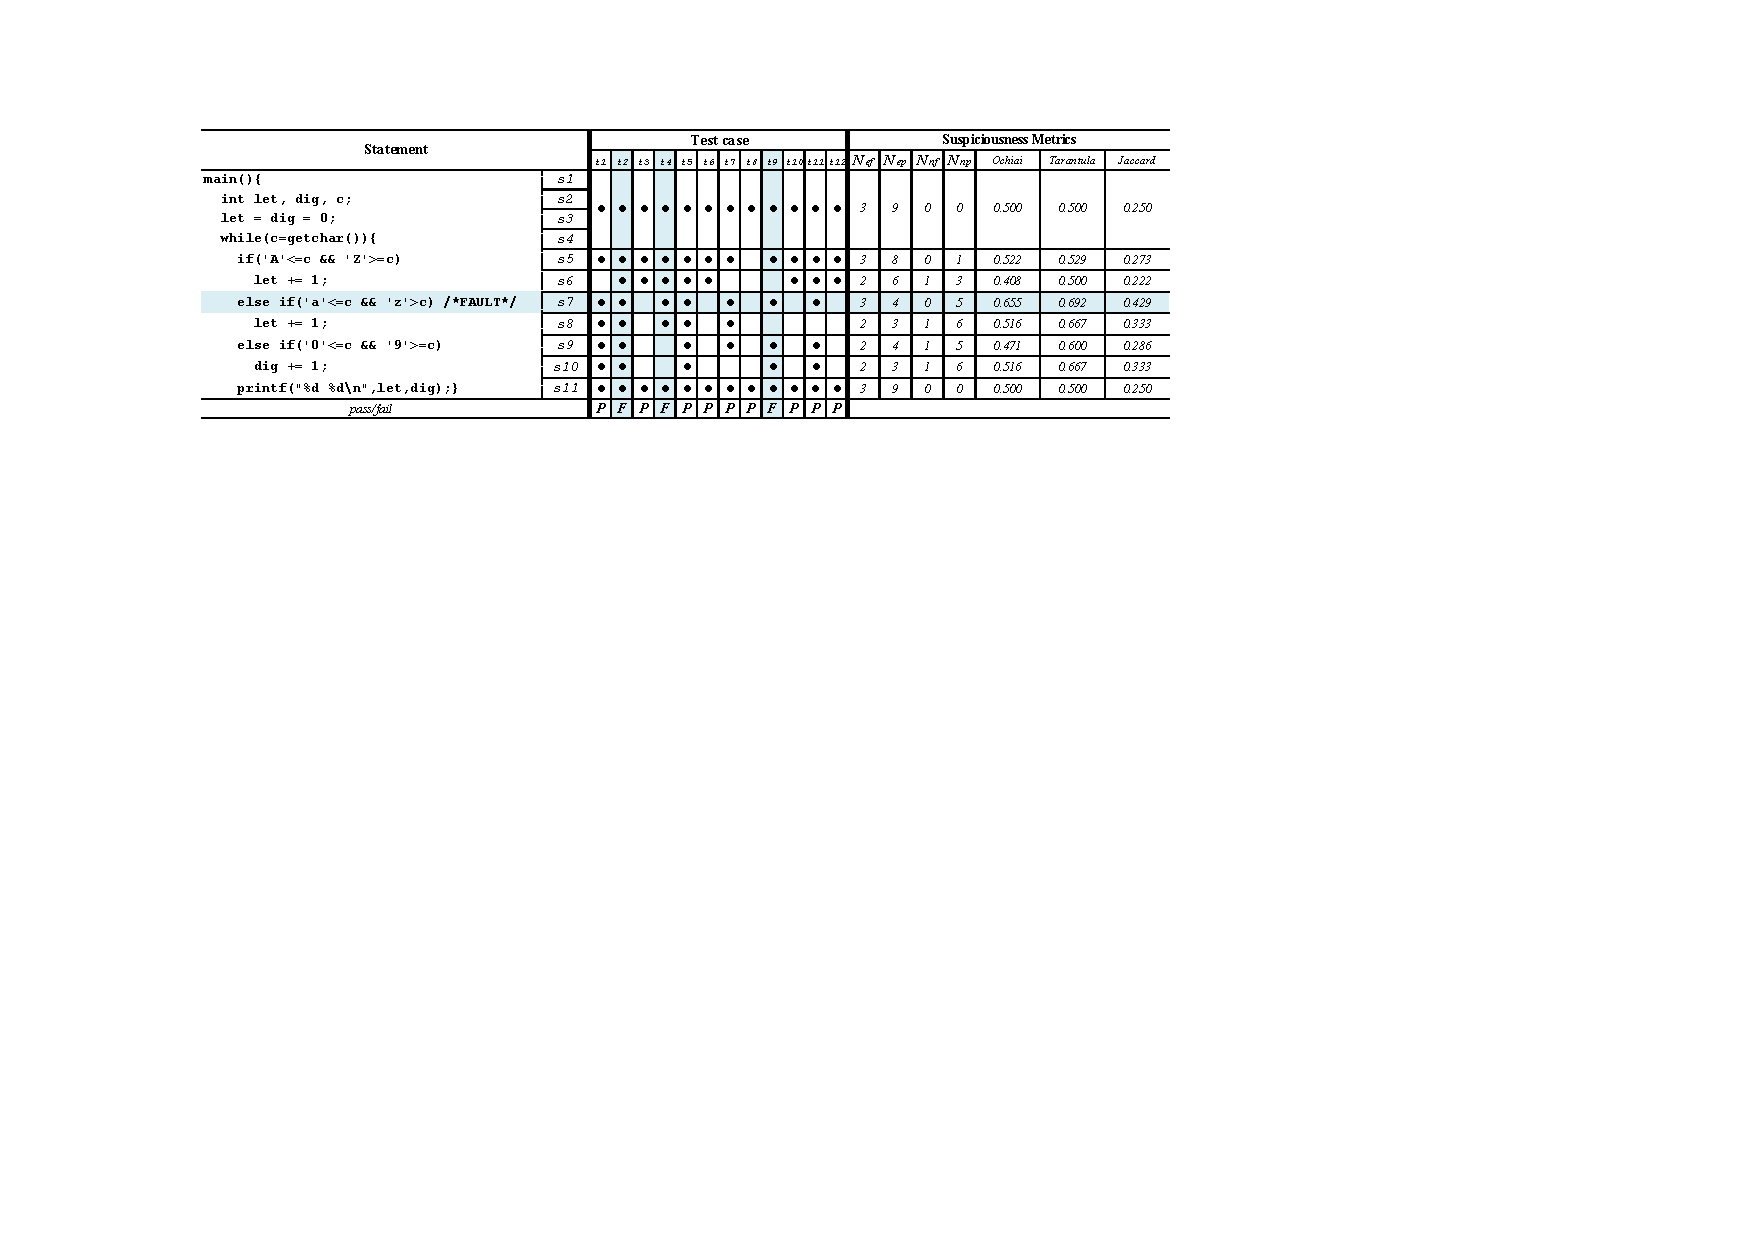
\includegraphics[width=12cm]{motivating_example.pdf}
  }
  \subfigure[Evolution of Suspiciousness Scores with Test Cases Selected by our approach]{
    \label{tab:dms_evo}
    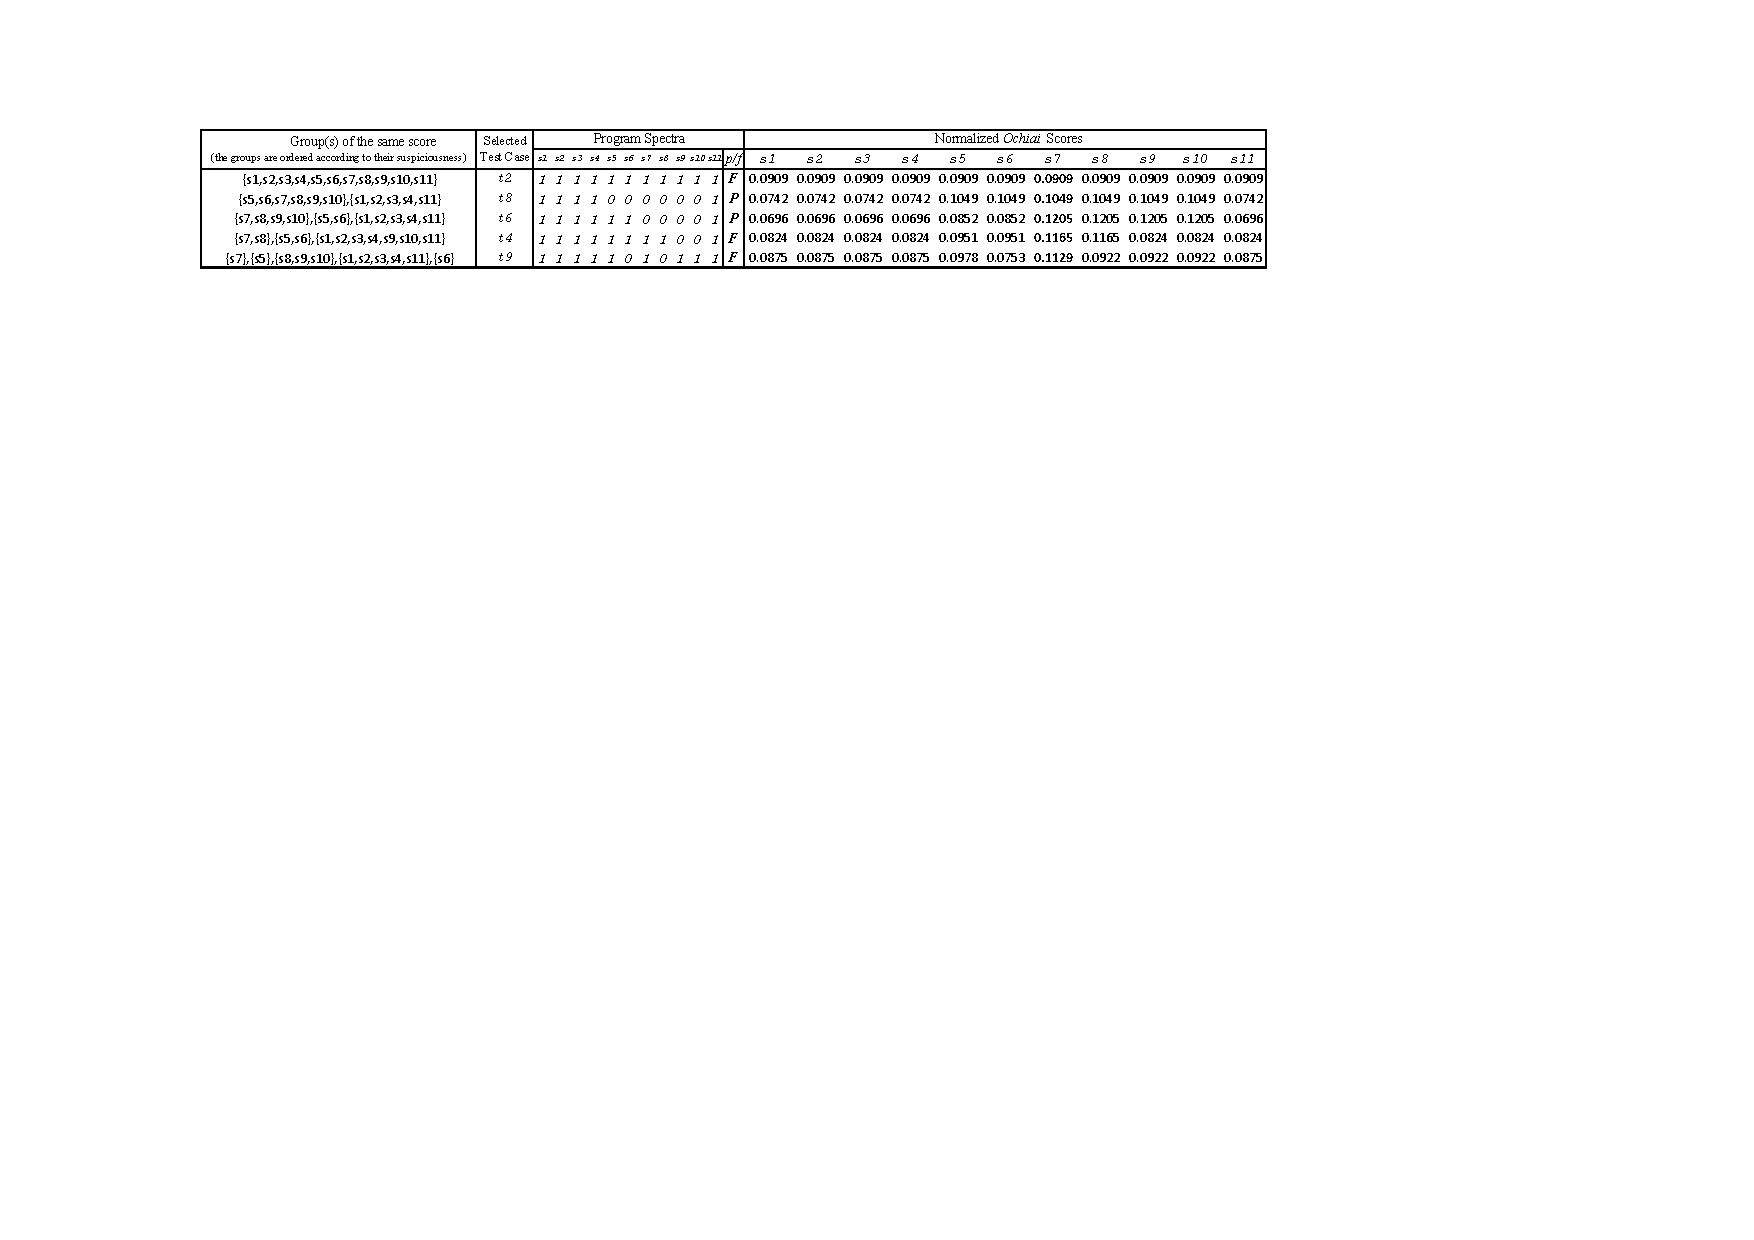
\includegraphics[width=12cm]{our_table.pdf}
  }
  %\vspace*{-16pt}
  \caption{Running Example}
  \label{fig:motiv-example}
\end{figure}

% Present key technical points
In this paper, we propose the concept of {\em diversity maximization speedup} ({\sc Dms}) and an associated test case prioritization strategy to minimize the human effort needed to label test cases while maintaining the effectiveness of existing spectrum-based fault localization techniques. The concept is based on our observation that when given sufficient test cases, an effective fault localization technique would assign a unique suspiciousness score to most program elements (e.g., a function, a statement, a branch, or a predicate), and high scores to faulty elements and low scores to non-faulty ones. We thus design {\sc Dms} to {\em speedup the changing process of the suspiciousness scores} generated by a fault localization technique {\em by using as few test cases as possible}.

This concept can be applied to both single-fault and multi-faults programs to reduce human efforts required for labelling test cases. On the other hand, the amount of reduction achieved by the concept can be different for single-fault and multi-faults scenarios. We present detailed experiments and comparison in Section~\ref{sec.experiment}. When we describe the intuition of this concept and the algorithmic details for realizing the concept, we do not explicitly distinguish these two scenarios from each other.

\subsection{Running Example}

%Essentially, {\sc Dms} aims to use as few test cases as possible to quickly exhibit different characteristics among different program elements and help fault localization techniques to discriminate fault elements from non-faulty ones. Then, the human labeling effort is only needed for the much reduced test cases.
Figure~\ref{motiv_example} and~\ref{tab:dms_evo} illustrate how our concept helps reduce the number of test cases for effective fault localization.

There are 11 statements $s_{1}...s_{11}$ in the program in Figure~\ref{motiv_example} (adapted from previous papers \citep{Gonzalez-SanchezPAGG11,JiangCT11}), where $s_{7}$ is faulty. Suppose the program has 12 test cases $t_{1}...t_{12}$. A dot for a statement under a test case means the corresponding statement is executed (or hit) in the corresponding test case. The collection of such dots (or represented as sequences of \texttt{\textit{1}} and \texttt{\textit{0}} as shown in Figure~\ref{tab:dms_evo}) are called {\em program spectra}. With the spectra for all of the test cases and their pass/fail information, fault localization techniques may calculate various suspiciousness scores for each of the statements and rank them differently. In this case, three well-known techniques, {\em Ochiai}~\citep{Abreu:2009.jss}, {\em Tarantula}~\citep{JH05}, and {\em Jaccard}~\citep{Abreu:2009.jss} all rank $s_{7}$ as the most suspicious statement (the last three columns in the highlighted row for $s_{7}$ in Figure~\ref{motiv_example}). However, the fault localization techniques can in fact achieve the same effectiveness (i.e., ranking $s_{7}$ as the top suspicious one) with much fewer test cases when our concept is applied.

Use {\em Ochiai} as an example. First, we select an initial small number of test cases ($t_{2}$ in the example). After a programmer labels the execution result of $t_{2}$, {\em Ochiai} can already assign suspiciousness scores to each statement, although the ranks are not accurate (as in the last 11 columns of the row for $t_{2}$ in Figure~\ref{tab:dms_evo}). Then, our approach calculates the potential rank changes that may be caused if a new test case is used by {\em Ochiai}, and selects the next test case with the maximal change-potential ($t_{8}$ in our case) for manual labeling. With a label for $t_{8}$, {\em Ochiai} updates the suspiciousness scores for the statements (as in the last 11 columns of the row for $t_{8}$). Repeating such a process three more times, test cases $t_{6}$, $t_{4}$ and $t_{9}$ are added, and {\em Ochiai} can already rank $s_{7}$ as the most suspicious statement. Thus, our approach helps {\em Ochiai} to effectively locate the fault in this case with only five test cases, instead of 12. Section~\ref{sec.problem} and~\ref{sec.approach} present more details about our approach.

\subsection{Contributions}

We have evaluated our approach on five real {\em C} programs and seven Siemens test programs from the Software-artifact Infrastructure Repository (SIR~\citep{doESE05}).
In total, we analyze 411 faults. 254 of them are in single-fault versions from these 12 programs, while the other 157 faults are in 173 versions of 8 of these programs.
The results demonstrate that our approach significantly outperforms existing test case selection methods for fault localization.

%\vspace{-5pt}
\begin{enumerate}
	\setlength{\parskip}{0pt}%
    \setlength{\itemsep}{3pt}%
	\item Given a target fault localization accuracy, our approach can significantly reduce the number of test cases needed to achieve it. In particular, we compare with several state-of-the-art test case prioritization strategies, including coverage-based (e.g., {\sc Stmt-Total}~\citep{RUCH01,SEAGMGR01}, {\sc Art}~\citep{JiangZCT09}), fault-exposing potential based~\citep{RUCH01}, and {\em diagnostic prioritization}~\citep{Alberto2011,Gonzalez-SanchezPAGG11,JiangCT11}, and our approach achieves, on average, test case reduction rates from
10\% to 96\% for single-fault programs, and 6\% to 67\% for multi-faults programs.
	\item Given a maximum number of test cases that a programmer can manually label (i.e., given a fixed number of test cases to be used for fault localization or a testing budget), {\sc Dms} can improve the accuracy of fault localization and thus helps reduce the amount of code programmers need to investigate to locate faults and reduce testing and debugging cost. In comparison with other test case selection techniques, we show, with Wilcoxon signed-rank test~\citep{WF1943} at 95\% confidence level, that the cost saving achieved by {\sc Dms} is statistically significant on real-life programs.
\end{enumerate}

\subsection{Paper Outline}

% Paper structure
The rest of this paper is organized as follows: Section~\ref{sec.prelim} describes fault localization and test case prioritization techniques that we use in our study. Section~\ref{sec.problem} formally introduces the problem we address. Section~\ref{sec.approach} presents our approach in detail. Section~\ref{sec.experiment} presents our empirical evaluation. Section~\ref{sec.related} describes more related works.
Finally, Section~\ref{sec.conclusion} concludes with future work.


%\vspace{-4pt}
\section{Preliminaries}\label{sec.prelim}
 In this section, we summarize relevant materials on software fault localization and test case prioritization that we use in our empirical evaluation.

\subsection{Fault Localization}\label{sec.prelim.fault_local_test_gen}

Spectrum-based fault localization aims to locate faults by analyzing program spectra of passed and failed executions. A program spectra often consists of information about whether a program element (e.g., a function, a statement, or a predicate) is hit in an execution.
%and how many times it is hit.
Program spectra between passed and failed executions are used to compute the suspiciousness score for every element. All elements are then sorted in descending order according to their suspiciousness for developers to investigate. Empirical studies \citep[e.g.][]{NainarCRL07,JH05} show that such techniques can be effective in guiding developers to locate faults. \cite{DBLP:conf/issta/ParninO11} conduct a user study and show that by using a fault localization tool, developers can complete a task significantly faster than without the tool on simpler code. However, fault localization may be much less useful for inexperienced developers.

The key for a spectrum-based fault localization technique is the formula used to calculate suspiciousness.
Table~\ref{table_all_techniques} lists the formulae of three well-known techniques: {\em Tarantula}~\citep{JH05}, {\em Ochiai}~\citep{Abreu:2009.jss},
and {\em Jaccard}~\citep{Abreu:2009.jss}. Given a program element $s$,
$N_{ef}(s)$ is the number of {\em \textbf{f}ailed} executions that {\em \textbf{e}xecute} $s$;
$N_{np}(s)$ numerates {\em \textbf{p}assed} executions that do {\em \textbf{n}ot} hit $s$;
by the same token, $N_{nf}(s)$ counts {\em \textbf{f}ailed} executions that do {\em \textbf{n}ot} hit $s$
and $N_{ep}(s)$ counts {\em \textbf{p}assed} executions that {\em \textbf{e}xecute} $s$.


\begin{table}[!h]
	\caption{Spectrum-based fault localization}
%    \scriptsize
        \centering
{
        \renewcommand{\arraystretch}{1.5}
        \begin{tabular}{l l l c} \hline
        Name &\quad& Formula \\ \hline\hline% \\ [-1.5ex]
        {\em Tarantula} &\quad&  $\dfrac{\frac{N_{ef}(s)}{N_{ef}(s) + N_{nf}(s)}}{\frac{N_{ef}(s)}{N_{ef}(s) + N_{nf}(s)} + \frac{N_{ep}(s)}{N_{ep}(s) + N_{np}(s)}}$ \\ [1ex] \\ [-1.5ex]
        {\em Ochiai} &\quad&  $\dfrac{N_{ef}(s)}{\sqrt{(N_{ef}(s)+N_{nf}(s))\cdot(N_{ef}(s)+N_{ep}(s))}}$ \\ [1ex] \\ [-1.5ex]
		{\em Jaccard} &\quad&  $\dfrac{N_{ef}(s)}{N_{ef}(s)+N_{nf}(s)+N_{ep}(s)}$ \\ \hline
        \end{tabular}
}
    \label{table_all_techniques}
\end{table}

\noindent{\bf Example.} Each column for $t_{i}$ in Figure~\ref{motiv_example} is a spectrum. The columns $N_{ef}$, $N_{ep}$, $N_{nf}$, and $N_{np}$ can thus be calculated from the spectra.
%in Figure~\ref{motiv_example} is a code snippet~\citep{Gonzalez-SanchezPAGG11,JiangCT11} that counts character with one seeded fault.
%We mutate the predicate in line 7 ($s7$ \texttt{`z'$>=$c} $\rightarrow$ \texttt{`z'$>$c}. As a result, test case with at least one \texttt{`z'} character will get a wrong output.
The suspiciousness scores of {\em Tarantula}, {\em Ochiai}, and {\em Jaccard} for each statement are then calculated based on the formulae in Table~\ref{table_all_techniques}.

%\vspace{0.2cm}
%\begin{center}
%\begin{tabular}{|l|c|}
%\hline {\bf Measure} & {\bf Suspiciousness}\\
%\hline {\em Ochiai} & 0.548\\
%\hline {\em Tarantula} & 0.563\\
%\hline {\em Jaccard} & 0.3\\
%\hline
%\end{tabular}
%\end{center}

%
%\begin{figure*}[!htbp]
%    \centering
%    \includegraphics[width=17cm]{problem.pdf}
%    \caption{Post-Mortem Analysis and Real Scenario}
%    \lx{May use this figure in the Intro as part of our motivation. Is it too big though?}
%    \label{fig:problem}
%\end{figure*}
%


\subsection{Test Case Prioritization}\label{sec.prelim.test_prior}

%This section introduces test case prioritization techniques.
\cite{RUCH01} define the problem of test case prioritization  as follows:

\begin{definition}[{\bf Test Case Prioritization}]
Given
(1) $T$, a set of test cases, (2) $PT$, the set of permutations of $T$, and (3) $f$, a function mapping $PT$ to real numbers, the problem is to find a permutation $p \in PT$ such that:
%\begin{center}
	$\forall{p' \in PT}. f(p) \geq f(p')$.
%\end{center}
\end{definition}

%\vspace{-4pt}
In this definition, $PT$ represents the set of all possible orderings of $T$; $f$ is an award function indicating the value for each ordering. The higher the value, the better it is. For easier implementation, award functions in the literature are often defined as a priority function mapping test cases to real numbers, and then the optimal permutation is simply to sort the test cases in descending order according to their values. The key for a test case prioritization technique to be effective is to design a priority function that assigns appropriate priority to the test cases under given situations.
%In the context of regression testing, $f$ can be a measure about the coverage rate of desired program elements. developers want to detect faults as early as possible, and thus the prioritization goal is to select test cases are to be run first such that faults are found earlier. Specifically, given two ordered sets of test cases $p$ and $p'$, if $p'$ reveals fault earlier than $p'$, then $f(p) \geq f(p')$.
The following subsections highlight some test case prioritization techniques that we compare with our approach.

%\vspace{-4pt}
\subsubsection{Coverage Based Prioritization}

\textbf{\textsc{S{\scriptsize TMT}-T{\scriptsize OTAL}}}~\citep{RUCH01} is a test case prioritization strategy that assigns higher priorities to
a test case that executes more statements in a program.
\textbf{S{\scriptsize TMT}-A{\scriptsize DDTL}}~\citep{RUCH01} extends \textsc{Stmt-Total} by selecting next test case that covers more statements
that have not been covered by previously selected test cases.
{\em Adaptive Random Test Prioritization} ({\bf A{\scriptsize RT}})~\citep{JiangZCT09} starts by randomly selecting a set of test cases
that achieves maximal coverage, and then sort the unlabeled test cases based on their {\em Jaccard distances} to previous selected test cases.
Among its several variants, {\bf A{\scriptsize RT}-M{\scriptsize IN}} was shown to be the best test case prioritization strategy~\citep{JiangZCT09}.
However, recent study~\citep{DBLP:conf/issta/ArcuriB11} shows that \textsc{Art} may not be effective when the failure rate is low and the high distance calculations cost might overshadow the reduction on test execution times.

%\vspace{-4pt}
\subsubsection{Fault-Exposing Potential Based Prioritization}
\textbf{\textsc{F{\scriptsize EP}-A{\scriptsize DDTL}}}~\citep{RUCH01} aims to sort test cases so that the {\em rate of failure detection}
of the prioritized test cases can be maximized. To reduce the need for test oracles, the rate of failure detection is approximated by the
{\em fault-exposing potential} (\textsc{Fep}) of a test case, which is in turn estimated based on program {\em mutation analysis}~\citep{RGHamlet1977}:
each program element $s_j$ is mutated many times and
the test case $t_i$ is executed on each mutant; the \textsc{Fep} of $t_i$ for $s_j$ ($\textsc{Fep}_{ij}$) is calculated as
the ratio of mutants of $s_j$ detected by $t_i$ over the total number of
mutants of $s_j$; then, the \textsc{Fep} of $t_i$ ($\textsc{Fep}_i$) is the sum of the FEP of $t_i$ for all elements ($\sum_{j}\textsc{Fep}_{ij}$).

%\vspace{-4pt}
\subsubsection{Diagnostic Prioritization}\label{subsubsec.dp}
\begin{comment}
There are many techniques proposed to automatically generate a large number of test inputs. However, there are only a few methods that could automatically generate test oracles which are often limited to a certain family of failures, e.g.,~\citep{Artzi2010,Xie06}. In post-mortem study, test oracles can be obtained by running test cases on the correct program (see Figure~\ref{fig:problem}(A)). In practice, however, the code base contains faults and developers are not aware of its location unless testing and debugging are performed. Therefore, the fault-free version of the program is absent and testers have to manually create test oracles for each input, or check the correctness of program output one by one, both of which are laborious (see Figure~\ref{fig:problem}(B)).

Diagnostic prioritization is proposed to deal with this problem. Diagnostic prioritization select and prioritize a relatively smaller subset of test cases and ask users to label the test outcome. The goal of test case prioritization and diagnostic prioritization is different though; while test case prioritization is often employed to reduce the amount of time needed to run all tests, diagnostic prioritization would like to reduce the number of test cases that need manual labeling and yet optimize fault localization accuracy. The problem of running too many test cases is not important in diagnostic prioritization as the key issue to be solved is the lack of test cases (with available oracles). We define this problem in Definition~\ref{defn:diagnosticpriori}.

\subsubsection{Existing Methods}
\end{comment}

%Jiang \etal
\citet{JiangCT11} investigate the effects of previous test case prioritization techniques on fault localization and find that coverage-based techniques may be insufficient since the prioritized test cases may not be useful in supporting effective fault localization.
%\textbf{Information Gain-based Approach.}
\cite{Gonzalez-SanchezPAGG11} use the concept of {\em diagnostic distribution} that represents the probability of a program element to be faulty, which is then estimated by {\em Bayesian inference} based on previous selected test cases, and in their tool named \textbf{S{\scriptsize EQUOIA}}, sort test cases so that the information entropy of the diagnostic distribution can be minimized.
%
%use of information gain as prioritizing metric which select trace
%based on the entropy of {\em diagnostic distribution}. In their method(\textsc{Sequoia})
%they estimate the probability of a {\em diagnosis}(program element $d_k$)
%containing fault $Pr(d_k)$ by the {\em Bayesian inference}.
%They also use a heuristic to adjust the probability.
%Generally speaking, each time when an element $d_k$ appears in failed trace,
%their method increase $Pr(d_k)$, otherwise, when $d_k$ is executed by passed trace
%or absent in failed trace, their method decreases $Pr(d_k)$.
%
%Based on the diagnostic distribution, their method always selects the test cases that leads to the
%minimal information entropy.
%
%\textbf{Ambiguity Group Reduction.}
Soon after, \cite{Alberto2011} propose another strategy
called {\em Ambiguity Group Reduction} to sort test cases.
%based on {\em Dynamic Basic Block}(\textsc{Dbb})~\citep{baudry06a}.
In their tool named \textbf{R{\scriptsize APTOR}}, program elements having the same spectrum record are considered to be in the same ambiguity group (\textsc{Ag}),
and {\sc Raptor} aims to select next test case that would maximize the number of ambiguity groups while trying to minimize the deviation on the sizes of the ambiguity groups.

\subsubsection{Practical Usage}

To use the above mentioned test case prioritization techniques in practice, a program needs to be instrumented first and executed with test cases to collect the program spectra (execution traces) of the test cases. Then, developers can apply one of the test case prioritization techniques to select top-$n$ ranked test cases, and manually judge whether each of the test cases passes or fails. Based on these selected test cases and their corresponding labels (passed or failed), a fault localization technique \citep[e.g.][]{NainarCRL07,JH05} can then be applied to locate faults. Our test case prioritization technique in this paper can also be applied in the same fashion as the above mentioned test case prioritization techniques.


%\vspace{-4pt}
\section{Problem Definition}\label{sec.problem}

In this section we show a motivating example and formally introduce our approach: {\em \textbf{D}iversity \textbf{M}aximization \textbf{S}peedup} (\textsc{Dms}). \textsc{Dms} employs trend analysis to give priorities to test cases that can quickly increase the diversity of suspiciousness scores generated by fault localization techniques for various program elements.
%It employs trend analysis to speedup the diversification process by identifying promising program elements that are likely to increase diversity as more test cases that execute them are selected.
In the subsections, we illustrate its intuition and formally define it as a variant of test case prioritization.
%show a motivating example and describe the details of our approach.

\subsection{Running Example Revisited}\label{sec.motive}



\begin{figure}[tbp]
    \centering
%    \vspace{-0.9cm}
    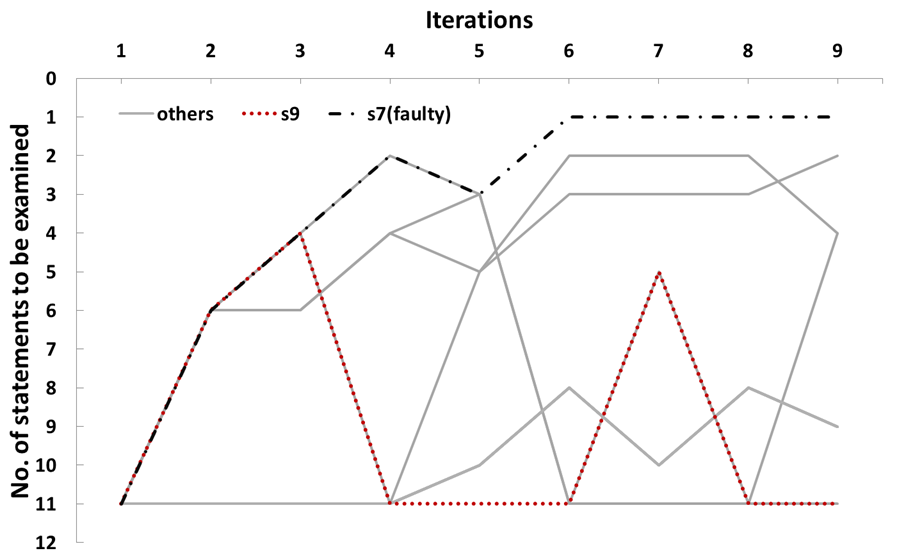
\includegraphics[width=12cm]{motive_1.png}
   % \vspace{-0.8cm}
    \caption{Motivating Example}
    \label{fig:motive_1}
\end{figure}

We use the running example (Figure~\ref{motiv_example}) to explain the intuitions for
\textsc{Dms}. With sufficient test cases, an effective fault localization technique is more likely to assign high suspiciousness scores to faulty program elements while assigning low scores to non-faulty elements, and each element should be assigned a unique rank according to their suspiciousness scores to facilitate further investigation (such as the scores shown in the last three columns in Figure~\ref{motiv_example}).

With fewer test cases, a fault localization technique may not be able to achieve an effective ranking. Figure \ref{fig:motive_1} shows the evolution trend of the ranks of the running example's program statements based on their {\em Ochiai}~\citep{Abreu:2009.jss} scores as test cases are added one by one. The test cases are added by \textsc{Raptor} which is the existing best approach in the literature~\citep{Alberto2011} for selecting test cases for fault localization. In this figure, the horizontal axis represents the number of iterations to select test cases. In each iteration, one test case is picked from the unlabeled test case pool $T_\mathcal{U}$.
The vertical axis is the rank
of a statement sorted based on suspiciousness.\footnote{\scriptsize Program elements with the same suspiciousness score are assigned the same {\em low} rank since developers are expected to investigate all of the elements having the same score if they are ever going to investigate one. For example, if statements $s_{1}$, $s_{2}$, $s_{3}$ have the highest suspiciousness score, then the ranks of the 3 statements are all 3.} Each line in the figure depicts the evolution of the suspiciousness rank for one specific statement. For example, $s_{7}$ (the faulty statement) is ranked $11^{th}$ in the first iteration, and $6^{th}$ in the second iteration.

This figure shows that the ranks of different statements may evolve in different ways as more test cases are added. Specifically, some statements keep rising in general (e.g., $s_{7}$); some others oscillate back and forth (e.g., $s_{9}$).
Ideally, we should only use test cases that could enable a fault localization technique to assign elements the scores close to the final score when all test cases are used.
Comparing to the changes of $s_{7}$, the oscillation of $s_{9}$ is less important as its final rank is the same as its initial rank.
Thus, when we add test cases, we should look for test cases that could offer more {\em changing opportunities} to ``promising'' elements like $s_{7}$ (with clear trend) instead of $s_{9}$ so that the ranks (for both $s_{7}$ and $s_{9}$) may quickly approach their final position.

\begin{comment}
Observing Figure \ref{fig:motive_1} we can see the ranks of different statements evolve in different ways as more test cases are added. The ranks of some statements decreases gradually (e.g., $s_{7}$'s rank), while the ranks of some elements oscillates back and forth (e.g., $s_{9}$'s rank). Elements whose ranks change much are interesting as they correspond to the increase in the diversity as more test cases are added.

\end{comment}

The following questions prompted us to define {\sc Dms}:

%\vspace{-4pt}
\begin{enumerate}
\item Can we analyze the change trend of every program element and identify ``promising'' elements with {\em high change potentials} (i.e., elements whose ranks are likely to change much in a stable way)?
%\vspace{-2pt}
\item For program elements having high change potentials, can we select appropriate test cases to speed up their rank-changing process so that these elements can reach their final ranks faster (i.e., with fewer test cases)?
\end{enumerate}

%\vspace{-6pt}
\subsection{Formal Definition of DMS}

%\vspace{-6pt}
\begin{definition}[{\bf Diversity Maximization Speedup}]
Given (1) $T$, a set of test cases, (2) $PT$, the set of permutations of $T$, and (3) $k$, a positive integer, we use $p^k$ to represent a permutation $p\in PT$ truncated at length $k$, and $PT^k$ to represent all such truncated permutations (i.e., $PT^k=\{p^k|p\in PT\}$).

Then, with $f$, a function mapping $PT^k$ to real numbers, the problem of DMS is to find a permutation $p \in PT$ such that:
%\begin{center}
	$\forall{p_i^{k} \in PT^{k}}.$	$f(p^{k}) \geq f(p_i^{k})$, for the given $k$.
%\end{center}
\label{defn:diagnosticpriori}
\end{definition}

In Definition~\ref{defn:diagnosticpriori}, $f$ is an award function indicating the value of an ordering in $PT^{k}$, which in our case, would be the effectiveness of a fault localization technique based on $k$ labeled test cases.
%, which is a set of test cases of size $k$. Without the loss of generality, the definition assumes
%that higher award values are preferable to lower ones.
The number $k$ can be used as a labeling budget, indicating the number of test cases developers are willing to label for fault localization.
%Fault localization techniques would analyze traces corresponding to the execution of these test cases and rank program elements based on suspiciousness. Developers can then browse this list and inspect program elements one-by-one based on their suspiciousness. Thus, the goal is to minimize developer's cost in browsing the list of program elements to find the location of the bug. Specifically, given two ordered sets of test cases $p$ and $p'$, if by analyzing $p$, the fault localization tool can put the buggy program element higher in the suspiciousness list than the corresponding list produced by analyzing $p'$, then $f(p) \geq f(p')$.
Thus, the goal for {\sc Dms} is to quickly maximize the effectiveness of fault localization techniques with at most $k$ labeled test cases.


%\vspace{-4pt}
\section{Approach Details}\label{sec.approach}


In this section we answer the two questions raised in Section~\ref{sec.motive} to conceptualize \textsc{Dms}.

\subsection{Identify High Change-potential Elements}

In order to evaluate the change potential of program elements, we first represent program element's rank changes as time series data points. We then fit the points to a linear model using regression analysis. The regression coefficient of the model and the error (i.e., discrepancy between the model and the real points) are used as proxy to identify program elements with high change potentials. More details are described as follows.

\vspace{0.2cm}
\noindent{\em Representative Time Series Construction.} We capture changes in the ranks of a program element as a series of {\em trend units}:

\begin{enumerate}
%	\setlength{\parskip}{0pt}%
    \setlength{\itemsep}{3pt}%
	\item When the rank of the program element decreases, its current trend unit is \texttt{[+]}.
	\item When the rank of the program element increases, its current trend unit is \texttt{[-]}.
	\item If the element's rank stays the same, its current trend unit is \texttt{[0]}.
\end{enumerate}

For example, the ranks of statement $s_{8}$ in different iterations and its corresponding trend units are listed in Table \ref{tab:trend_example}. This series of trend units is further converted to a series of points $<x_{i},y_{i}>$, where $x_{i}$ represents the iteration number, and $y_{i}$ represents cumulated changes in program ranks at iteration $i$. We set $y_{0}$ as 0. When the trend in iteration $i$ is {\bf \texttt{[+]}}, $y_{i} = y_{i-1} + 1$.
If the $i$-th trend is {\bf \texttt{[-]}}, $y_{i} = y_{i-1} - 1$, otherwise, if the trend does not change({\bf \texttt{[0]}}) then $y_{i} = y_{i-1}$. We refer to this series of points as the {\em evolution trend} of the corresponding program element.

\begin{table}[t]
%	\small
	\centering
	\caption{Evolution Trend of $s_8$.}
	\renewcommand{\arraystretch}{1.5}
	\newcolumntype{C}{>{\centering\arraybackslash}m{0.45cm}<{}}
	\begin{tabular}{cCCCCCCCC}
		\hline
		Iteration ($x_{i}$) &1 &2 &3 &4 &5 &6 &7 &... \\
		\hline\hline
		Rank &11 & 6 & 4 &2 &3 &11 & 5 & ... \\
		Trend ($\mathcal{T}$) & {\bf}&{\bf\texttt{[+]}}&{\bf\texttt{[+]}}&{\bf\texttt{[+]}}&{\bf\texttt{[-]}}&{\bf\texttt{[-]}}&{\bf\texttt{[+]}}&... \\
		$y_{i}$ & 0 & 1 & 2 & 3 & 2 & 1 & 2 & ... \\
		\hline
	\end{tabular}
%	\vspace*{-8pt}
    \label{tab:trend_example}
\end{table}


\vspace{0.2cm}
\noindent{\em Linear Model Construction.} Then we use {\em linear regression analysis}~\citep{GrIy94} to model the trend of each program element. Each trend is modeled as a linear equation:

\begin{equation}
	y_{i}=\beta_{1}\cdot x_{i} + \beta_{0} + \epsilon_{i}
\end{equation}

\begin{comment}
\hide{
where the parameter $\beta_1$ is estimated by:
\begin{equation}
	\hat{\beta}_{1} = \frac{\sum\limits_{i}{(x_{i}-\bar{x})\cdot(x_{i}-\bar{x})}}{\sum\limits_{i}{(x_{i}-\bar{x})^2}}
\end{equation}
the error of estimation $\hat{\beta}_{1}$ is given by:
\begin{equation}
	\hat{\sigma}_{\beta_{1}} = \hat{\sigma}_{\epsilon}\sqrt{\frac{1}{\sum\limits_{i}{(x_i-\bar{x}^2)}}}
\end{equation}
in the equation, $\hat{\sigma}_{\epsilon}$ is the estimate of constant variance of error term, which is
defined by:
\begin{equation}
	\hat{\sigma}_{\epsilon} = \frac{1}{N-2} \cdot \sum\limits_{i}{e_{i}^{2}}
\end{equation}
where $e_{i} = y_{i} - \hat{y}_{i} $ which is the error between the actual value and predicted value.
}
\end{comment}

\vspace{0.2cm}
\noindent{\em Change Potential Computation.} In order to speed up the overall evolution process, our approach needs to select next test case that keeps elements with monotonic trends (high change-potential trends) evolving their rankings. In other words, we do not care about changing elements' ranking with unstable trends. In order to identify those high change-potential elements, we need a metric to evaluate and compare trends of different elements. Here we define the change potential of a program element $d$ with the trend $\mathcal{T}_d$ as follows:

\begin{equation}
\label{eq:trend_metric}
	\mathcal{W}_{\mathcal{T}_d} =  \frac{| \hat{\beta}_{1} |}{\hat{\sigma}_{\beta_{1}}+1}
\end{equation}


\noindent
%where $\mathcal{T}_d$ is the estimated linear model for $y_i$ of the element $d$,
$\hat{\beta}_{1}$ is estimated by {\em least squares} and $\hat{\sigma}_{\beta_{1}}$ is the error of estimating $\beta_{1}$~\citep{GrIy94}. In this metric, the numerator is the absolute value of the trend slope and the denominator considers the fitness of the regression model which represents the deviation of the actual value from the regression model.
When the context is clear, we also use $\mathcal{W}_\mathcal{T}$ or $\mathcal{W}_d$ to represent the change potential of a trend or a program element.

\noindent\textbf{Rationale of Equation \ref{eq:trend_metric}:} We want to evolve the ranks of statements in a fast, monotonic way. In linear models, \textit{a fast changing monotonic trend should have a larger slope $\beta_1$ as well as a smaller deviation $\epsilon_i$ from the linear model.}
%In linear models, fast changing monotonic model has a bigger slope and thus gets a bigger numerator. Meanwhile a stable and monotonic trend has a smaller deviation from the linear model and thus gets a smaller denominator.
Using this metric in Equation 2 that uses the estimated slope in the numerator and the estimated deviation in the denominator, we may isolate trends that evolve in faster and more stable (less oscillation) ways. Table \ref{tab:trend_exp} shows a few sample trends and their change potentials according to Equation \ref{eq:trend_metric}.

\begin{table}[!htbp]
	\centering
%	\vspace*{-8pt}
	\caption{Trend examples and their potentials}
		\renewcommand{\arraystretch}{1.5}
%		\small
        \begin{tabular}{|cc|ccc|}
			\hline
			 \multicolumn{ 2}{|c|}{$\mathcal{T}$} &     $\hat{\beta}_{1}$ &      $\hat{\sigma}_{\beta_{1}}$ &  $\mathcal{W}_\mathcal{T}$ \\
			\hline\hline
			 {\bf \texttt{[+]}} &  {\bf \texttt{[+]}} &          1 &          0 &          1 \\
			\hline
			 {\bf \texttt{[+]}} &  {\bf \texttt{[-]}} &          0 &      0.577 &          0 \\
			\hline
			 {\bf \texttt{[+]}} &  {\bf \texttt{[0]}} &        0.5 &      0.289 &      0.388 \\
			\hline
			 {\bf \texttt{[0]}} &  {\bf \texttt{[0]}} &          0 &          0 &          0 \\
			\hline
		\end{tabular}
	\label{tab:trend_exp}
\end{table}

\subsection{Speed up the Rank Change Process}

After evaluating the program elements according to their change potentials, \textsc{Dms} will try to speed up the evolution trend of the program elements based on the change potential ($\mathcal{W}_{\mathcal{T}}$). First, program elements with the same suspiciousness scores are grouped together, they are termed as {\em suspicious groups} in this paper.\footnote{We call such groups as {\em suspicious groups} since we simply want to state the fact that every group may contain potentially suspicious elements. Some other studies \cite[e.g.][]{Alberto2011} call them {\em ambiguity groups} as that term may emphasize more on the fact that the elements in the groups have the same but ambiguous suspiciousness scores.} These suspicious groups are then assigned change-potential scores based on the change potentials of their constituent program elements. When new test cases are added, based on the actual program elements that get executed, some groups can be broken into two. When this happens, the diversity of the suspiciousness scores increases in most cases. The goal of \textsc{Dms} is to select a new test case that breaks a group into two sub-groups where the overall change potentials are maximized.

We calculate the potential of a group $g$ by summing up the potential of all program elements $d$ that
belongs to $g$.
\begin{equation}
\label{eq:elem_potential}
	\mathcal{W}_{g} = \sum\limits_{d \in g}\mathcal{W}_{\mathcal{T}_{d}}
\end{equation}

\noindent
where $\mathcal{W}_{\mathcal{T}_d}$ is the change potential of the program element $d$ based on the labelled execution trace profiles.

\noindent\textbf{Rationale of Equation \ref{eq:elem_potential}:} \textit{A group with high change-potential elements should be given a higher priority to break.}
We want to diversify the rankings of elements in the suspicious group that has a high change-potential score.
To identify those high change-potential groups, we measure the sum of change-potential scores of its member elements as in Equation~\ref{eq:elem_potential}.

The overall change-potential score of all suspicious groups ($G$) is calculated as follows:
\begin{equation}
	\mathcal{H}_G = \sum\limits_{g_{i} \in G}{ \mathcal{W}_{g_i}^{2} }\label{eq:groupset_potential}
\end{equation}

To evaluate an unlabeled trace $t$, {\sc Dms} calculates the difference between the overall change-potential score of the current groups $G$ ($\mathcal{H}_G$) and the overall change-potential score of all groups when $t$ is added to the pool of labeled test cases ($G \Leftarrow t$).
Since we want to stabilize the ranks of all program elements as quickly as possible with as fewer test cases as possible, we heuristically choose the test case that can maximize the difference and thus the reduction of change potentials as the next one for labeling.
\begin{equation}
	\operatorname*{arg\,max}_{t \in T_\mathcal{U}} \left\{ \mathcal{H}_G - \mathcal{H}_{(G \Leftarrow t)} \right\}\label{eq:select_metric}
\end{equation}

The new groups ($G \Leftarrow t$) and their change potential $\mathcal{H}_{(G \Leftarrow t)}$ can be estimated based on $t$'s spectrum (i.e., the set of program elements hit by $t$) even when the pass/fail label for $t$ is unknown. Given an existing suspicious group, if a newly added test case $t$ only covers a subset of the group elements, this group may be broken into two: one contains the elements hit by $t$, and the other contains the elements uncovered by $t$. Then, each subgroup inherits a portion of the original group's change potential proportional to its size. For example, suppose a group $g$ in $\mathcal{H}_{G}$ contains 2 elements, whose potentials are 0.4 and 0.6 respectively, and a new test case $t$ breaks $g$ into $g_{1}$ and $g_{2}$, each of which contains 1 element; then, the change potentials $\mathcal{W}_{g_1}$ and $\mathcal{W}_{g_2}$ are both $\frac{1}{2}\times(0.4+0.6) = 0.5$.

\noindent\textbf{Rationale of Equation \ref{eq:groupset_potential} and \ref{eq:select_metric}:} \textit{A test case that breaks more groups with higher change potentials should be given a higher priority.}
Equation \ref{eq:groupset_potential} measures the overall change potential score of all suspicious groups and its square form manifests the diversity of element ranks.
As an example, suppose there are two groups $g_{1}$ and $g_{2}$. Group $g_1$ has two high change-potential elements with change-potential score 0.3 and 0.4.
Group $g_{2}$ has two low change-potential elements with change-potential score 0.1 and 0.2.
According to Equation \ref{eq:groupset_potential}, $\mathcal{H}_G = (0.3+0.4)^{2} + (0.1 + 0.2)^2 = 0.58$. After choosing a test case that breaks $g_1$ only and does not change the change-potential score of any element, then according to Equation \ref{eq:select_metric}, the new change potential would be $0.3^{2} + 0.4^{2} + (0.1 + 0.2)^2 = 0.34$. However, if we choose another test case that breaks $g_{2}$ only and does not change the change-potential score of any element, the new change potential would be $ (0.3+0.4)^{2} + 0.1^{2} + 0.2^{2} = 0.54$. As a result, the test case that breaks the high change-potential group (\textit{i.e.,} $g_{1}$) leads to a larger decrease of the overall change potential and thus will be given a higher priority to be selected.

Note that \textsc{Dms} does not intentionally increase suspiciousness scores of promising statements that could lead to {\em confirmation bias}.
%More specifically,
\textsc{Dms} might make an initially promising statement become less suspicious if the statement is covered in the next selected trace and the trace is labeled as {\em pass}, or it is not covered in the next selected trace and the trace is labeled as {\em fail}.

\subsection{Overall Approach}

Before prioritization, all test cases will be executed on instrumented program versions and the corresponding traces would be collected.
Our approach (pseudocode in Algorithm~\ref{algo:DMS}) takes in a set of unlabeled traces $T_\mathcal{U}$ and the labelling budget $k$ (i.e., the maximum number of traces to be manually labeled), and outputs $k$ selected traces for manual analysis.
One failed trace ($t_{0}$ in Line 1) is also used as an input because a developer usually starts debugging only when at least one test fails,\footnote{If there is more than one test that fails, {\sc Dms} randomly selects one of them to begin with.} and fault localization techniques rarely produce meaningful results if all spectra consists of only passed executions.

To collect indicative trends for analyzing and speedup, at Lines 3-9 we first collect $w$ traces by one generic prioritization technique $\mathcal{P}$ and record evolution trend $\mathcal{T}_{d}$ for each program element $d$. This step is desirable since it helps bootstrap the trend analysis in our solution.
At Lines 12-24, we perform the second stage which speeds up the change process based on existing trends. Note that after selecting each test case $t$ in this stage, we will update the trend for all elements. $f_{T}$ represents a fault localization technique (e.g.,{\em Ochiai}), built based on the set of test cases $T$. $f_{T}(d)$ returns the suspicious score for the program element $d$.



\begin{algorithm}%[!htb]
{
\centering
%\vspace{0.2cm}
 
\hspace{-0.0cm}\parbox[l]{3.2in} {
{%\small
\begin {tabular}[t]{l}
\textbf{Procedure DiversityMaximizationSpeedup}\\
\textbf{Input:}\\
\quad $k$ - Maximum number of traces to be selected\\
\quad $w$ - Switching threshold\\
\quad $T_\mathcal{U}$ - Unlabeled trace set, where $|T_\mathcal{U}|> k$\\
\quad $t_0$ - Initial failed trace\\
\textbf{Output:}\\
\quad $k$ selected test cases prioritized\\
\textbf{Method:}\\
\end{tabular}
\begin{algorithmic}[1]
	\STATE $T_{tmp} \leftarrow \{<t_0, fail>\}$
	\STATE \textit{\texttt{//Bootstraping with prioritization technique}} $\mathcal{P}$
	\WHILE{$|T_{tmp}|\leq k$ \AND $\left| T_{tmp} \right| \leq w$}
		\STATE Select $t$ by $\mathcal{P}$
		\STATE $c \leftarrow$\texttt{\textbf{manual\_label}}($t$)
		\STATE $T_{tmp} \leftarrow T_{tmp} \cup \left\{\right.<t, c>\left.\right\}$; $T_\mathcal{U}\leftarrow T_\mathcal{U} \setminus \left\{t\right\}$
		\STATE $\forall d \in \mathcal{D}$, calculate suspicious score $f_{T_{tmp}}(d)$
		\STATE $\forall d \in \mathcal{D}$, update trend $\mathcal{T}_{d}$ based on $f_{T_{tmp}}(d)$
	\ENDWHILE
	\STATE $T_\mathcal{S} \leftarrow T_{tmp}$
	\STATE \textit{\texttt{//Speedup}}
	\WHILE{$|T_\mathcal{S}|\leq k$}
		\STATE $\forall d \in \mathcal{D}$, calculate $\mathcal{W}_{\mathcal{T}_{d}}$ by Equation \ref{eq:trend_metric}
		\STATE Select $t$ by Equation \ref{eq:select_metric}
		\STATE $c \leftarrow$\texttt{\textbf{manual\_label}}($t$)
		\STATE $T_{tmp} \leftarrow T_{tmp} \cup \left\{\right.<t, c>\left.\right\}$; $T_\mathcal{U}\leftarrow T_\mathcal{U} \setminus \left\{t\right\}$
		\STATE $\forall d \in \mathcal{D}$, calculate suspicious score $f_{T_{tmp}}(d)$
		\STATE $\forall d \in \mathcal{D}$, update $\mathcal{T}_{d}$ based on $f_{T_{tmp}}(d)$
		\STATE $T_\mathcal{S} \leftarrow T_\mathcal{S} \cup T_{tmp}$
		\IF {\texttt{\textbf{div}}($T_{tmp}$) cease growing}
			\STATE $T_{tmp} \leftarrow \{<t_0, fail>\}$
			\STATE $\forall d \in \mathcal{D}$, clear $\mathcal{T}_{d}$
		\ENDIF
	\ENDWHILE
	\STATE return $T_\mathcal{S}$
\end{algorithmic}
}
}
}
%\vspace{-0.2cm}
\caption{\small{Diversity Maximization Speedup}} \label{algo:DMS}
%\vspace{-0.0cm}
\end{algorithm}











In the pseudocode, \texttt{\textbf{manual\_label}}($t$) asks a user to check
the correctness of the outcome from the test case $t$. Procedure \texttt{\textbf{div}}($T$)
counts the number of unique suspicious scores (diversity) generated by $f_T$, which is defined as follows:
\begin{equation}
	\texttt{\textbf{div}}(T) = \left| \bigcup\limits_{d \in \mathcal{D}} \{f_{T}(d)\} \right|
\end{equation}

The diversity of small programs may reach the maximum after selecting a small number of test cases. To avoid random selection
after that happens, the pseudo-code at Lines 20-23 resets the set $T_{tmp}$
based on which the suspiciousness scores of all program elements are calculated. With this step, \textsc{Dms} can
continually choose test cases from $T_{\mathcal{U}}$ that maximally diversify suspicious scores calculated based on $T_{tmp}$.
Repeating the diversity selection process may help to confirm the previously selected test cases and make the final result more robust.

%\lx{merged with the last paragraph in "Example"}
%Table \ref{tab:dms_evo} shows the selected test cases for the motivating example using \textsc{Dms}.  \textsc{Raptor} needs five labeled traces (\texttt{$t_{8}$}$\rightarrow$\texttt{$t_{6}$}$\rightarrow$\texttt{$t_{4}$}$\rightarrow$\texttt{$t_{7}$}$\rightarrow$\texttt{$t_{9}$}) to
%rank the real fault ($s_{7}$) top in the check list (see Table \ref{tab:ag_evo}) based on maximal {\em Ambiguity Group Reduction}(see Section \ref{subsubsec.dp}), \textsc{Dms} only requires user to manually label four traces (\texttt{$t_{8}$}$\rightarrow$\texttt{$t_{6}$}$\rightarrow$\texttt{$t_{4}$}$\rightarrow$\texttt{$t_{9}$}).

%The delay between each round of query is short as the time complexity of computing suspiciousness score for all program elements $\mathcal{D}$ is $O(\left|\mathcal{D}\right|)$ and the time complexity of computing trend score is $O(\left|\mathcal{D}\right| \cdot k)$. Users can choose to stop the process when the cost budget is exhausted (e.g., when the number ($k$) of test cases a user is willing or able to label has been reached).

%Our approach greedily splits suspicious groups based on all previously labeled tests. This may lead to a non-optimal solution as defined by Definition 3.1, but it much simplifies our solution and our empirical study shows it produces promising results to save much human labeling effort, although it may not necessarily save machine time that is required to run all test cases.

%\vspace{0.2cm}
%\noindent{\it Example.}
\subsection{Example}
We describe step by step how \textsc{Dms} minimizes the number of test cases needed by {\em Ochiai} to locate
the fault in the running example in Figure~\ref{motiv_example} and Figure~\ref{tab:dms_evo}.

Since the example code snippet is quite small, there is no need to use a large number of initial test cases to bootstrap our trend analysis. %faulty element $s_{7}$ are ranked $1^{st}$ after selecting only a few traces using \textsc{Raptor}.
We set $w=1$ and only use one test case (in addition to $t_0$) for bootstrapping. In this example and our evaluation in Section~\ref{sec.experiment}, we use \textsc{Raptor}, one of the previously best techniques, in the bootstrapping process for better comparison.

Initially, users execute the program and expose a failure ($t_2$ in this example) in which all statements are covered.
Thus all statements get equal non-zero suspiciousness and constitute a suspicious group $g$. All non-zero suspicious groups compose a group set $G = \{g\}$.
{\sc Raptor} would then choose $t_8$\footnote{$t_8$ has the maximum ambiguity reduction values.} and ask developer to label ({\em pass} or {\em fail}).


After the bootstrapping stage, {\em Ochiai} updates the suspiciousness score for each statement based on the selected traces
and the existing suspicious group set are broken into \{$s_{1}$,$s_{2}$,$s_{3}$,$s_{4}$,$s_{11}$\} and \{$s_{5}$,$s_{6}$,$s_{7}$,$s_{8}$,$s_{9}$,$s_{10}$\}, they are
called $g_{1}$ and $g_{2}$ respectively.
At this time, the trend for the statements in $g_{1}$ is {\bf\texttt{[+]}}, because the ranks of these statements change from 11 to 6, while the trend for the statements in $g_{2}$
is {\bf\texttt{[0]}}, because their ranks are still 11.
The corresponding time series of the statements in $g_{2}$ are:
$y_{0} = 0$ and $ y_{1} = 1$. Applying equation \ref{eq:trend_metric}, we obtain the change-potential of the trend of the program elements in $g_{2}$ as 1.


We now calculate $\mathcal{H}_{G}$ for the current suspicious group set $G=\{g_{1},g_{2}\}$ according to Equation \ref{eq:elem_potential}:

\[\mathcal{H}_{G} = \mathcal{W}_{g_{1}}^{2} + \mathcal{W}_{g_{2}}^{2}  = (\sum_{d \in g_{1}}{0})^{2} + (\sum_{d \in g_{2}}{1})^{2} = 36\].

Now there are 10 candidate traces: $\{t_{i} | 1\leq~i~\leq~12 \wedge i\notin\{2,8\}\}$ to be evaluated. We will use each candidate trace $t_{i}$ to
break ties in $G$ ($G \Leftarrow t_{i}$). Then we calculate the score that evaluates the breaking effect: $\mathcal{H}_{(G \Leftarrow t_{i})}$.

For example, when evaluating $t_6$, $t_{6}$ covers $s_{1}$,$s_{2}$,$s_{3}$,$s_{4}$,$s_{5}$,$s_{6}$ and $s_{11}$, thus breaks suspicious $g_{2}$
into \{$s_{5}$,$s_{6}$\} and \{$s_{7}$,$s_{8}$,$s_{9}$, $s_{10}$\}, let us call them $g_{21}$ and $g_{22}$ respectively.
Now, the score $\mathcal{W}_{g_{21}} = \frac{2}{6} \times \mathcal{W}_{g} = 2$, $\mathcal{W}_{g_{22}} = \frac{4}{6} \times 6 = 4$.
So if choosing $t_{6}$, the score for $G$ is 

\[\mathcal{H}_{(G \Leftarrow t_{6})} = \mathcal{W}_{g_{21}}^{2} + \mathcal{W}_{g_{22}}^{2} = 20\]
And the reduction is 

\[\mathcal{H}_{G} - \mathcal{H}_{(G \Leftarrow t_{6})} = 36 - 20 = 16\].

In the same way, we evaluate all candidate traces and find that the reduction of $t_{6}$ is maximal, so we select $t_{6}$ as the next trace and ask developer to manually label $t_{6}$.
The developer then labels it as {\em ``pass''}.  After adding newly labeled trace $t_{6}$ into the selected trace set $T_{\mathcal{S}}$, we recalculate the suspicious score
of all program elements according to the current selected trace set. After calculation, the normalized suspicious score of the elements in \{$s_{5}$,$s_{6}$\} reduced from 0.1049 to 0.0852 and their ranks remains the same. The suspicious scores of
the elements in \{$s_{7}$,$s_{8}$,$s_{9}$,$s_{10}$\} increase from 0.1049 to 0.1205 and thus their ranks rises from 6 to 4. After that, the trends of program elements are updated. For example, the trend of elements in \{$s_{1}$,$s_{2}$,$s_{3}$,$s_{4}$,$s_{13}$\} becomes ({\bf\texttt{[0]}}{\bf\texttt{[0]}}), the trend
of the statements in \{$s_{5}$,$s_{6}$\} becomes ({\bf\texttt{[+]}}{\bf\texttt{[0]}}) and those in \{$s_{7}$,$s_{8}$,$s_{9}$,$s_{10}$\} corresponds to ({\bf\texttt{[+]}}{\bf\texttt{[+]}}).


Note that right now \{$s_{7}$,$s_{8}$,$s_{9}$,$s_{10}$\} gets the highest change-potential score and thus can get more chances to be broken up.
As shown in Table \ref{tab:dms_evo},
after three iterations,
\textsc{Dms} selects (\texttt{$t_{8}$}$\rightarrow$\texttt{$t_{6}$}$\rightarrow$\texttt{$t_{4}$}). In the next iteration, \textsc{Dms} chooses $t_{9}$ and breaks \{$s_{7}$,$s_{8}$\} and \{$s_{5}$,$s_{6}$\} which have greater change-potentials and consequently ranks $s_7$ the highest. Overall, {\sc Dms} only requires user to manually label four additional traces (\texttt{$t_{8}$}$\rightarrow$\texttt{$t_{6}$}$\rightarrow$\texttt{$t_{4}$}$\rightarrow$\texttt{$t_{9}$}).

As a comparison, \textsc{Raptor} always chooses the test case that maximally reduces the overall sizes of groups of statements that have the spectrum records (i.e., Ambiguity Group Reduction, c.f.\ Section~\ref{subsubsec.dp}). As shown in Table~\ref{tab:ag_evo}, \textsc{Raptor} effectively selects the same test cases as {\sc Dms} in the first four iterations; however, it chooses $t_{7}$ in the next iteration to break \{$s_{1}$,$s_{2}$,$s_{3}$,$s_{4}$,$s_{9}$,$s_{10}$,$s_{11}$\} and \{$s_{5}$,$s_{6}$\}, and it takes one more iteration to rank $s_7$ the highest.
%Because breaking these groups can get maximal overall group size reduction.
It thus requires users to label five additional test cases besides $t_2$ (\texttt{$t_{8}$}$\rightarrow$\texttt{$t_{6}$}$\rightarrow$\texttt{$t_{4}$}$\rightarrow$\texttt{$t_{7}$}$\rightarrow$\texttt{$t_{9}$}).


\subsection{Approach Complexity and Robustness}

The time and space complexity of our approach depend on many various factors. It takes linear time with respect to the number of iterations or test cases
we want to select, takes quadratic time with respect to the total number
of available test cases, takes cubic time with respect to the number of program elements, takes cubic time with respect to the number of suspicious
groups in each iteration. Our approach would also store all of the test spectra in
the memory for convenience. In comparison with the other existing approach {\sc Raptor}, the trend analysis step in our approach may be more computationally expensive. However, the step would still take short absolute amount of time since the number of selected test cases can be limited to tens or hundreds to achieve effective fault localization.

The results of our approach may not be deterministic either since there are random factors (e.g., the first failed test case to choose) and several user-defined parameters (e.g., the maximal number of test cases to select) employed in the approach. Thus, we repeat running our approach for multiple times in our evaluation to take average performance. The maximal number of test cases to select (i.e., $k$ in Algorithm \ref{algo:DMS}) and the switching threshold $w$ in the bootstrap phase would affect how much improvements our approach can achieve over other existing techniques, but they do not matter for the main focus of our evaluation, which is to evaluate whether Diversity Maximization Speedup ({\sc Dms}) is effective for reducing manual labelling effort and diagnostic cost. Although we expect different optimal $k$ and $w$ for different kinds of programs and faults, we use a consistent setting $k<=500$ and $w=10$ in our evaluation and would suggest potential users to starts with a small setting where they can tolerate the manual labelling cost.


%\vspace{-4pt}
\section{Empirical Evaluation}\label{sec.experiment}
In this section we present empirical evaluation that analyzes the impact of \textsc{Dms} on manual effort needed for test case labeling, and compares our approach with multiple previous test case prioritization methods.

In particular, our seek for answers to the following two research questions:

%\subsection{Research Questions}\label{sec.exp.rqs}

\begin{enumerate}[RQ1]
\item What is the effectiveness of \textsc{Dms} on single-fault programs?
\item What is the effectiveness of \textsc{Dms} on multi-fault programs?
\end{enumerate}

Section~\ref{sec.rq1} shows our experimental results that answer the first research question. Section~\ref{sec.rq2} presents answers to the second research question. Section~\ref{sec.exp.threats} describe the discussion and some threats to validity.


\subsection{RQ1: Single-Fault Programs}\label{sec.rq1}
Section~\ref{sec.exp.setup} gives details about our experimental setup for single-fault programs.
In Section~\ref{sec.exp.subject}, we introduce the subject programs used in our study. Sections~\ref{sec.exp.resultsA}~\&~\ref{sec.exp.resultsB} show the results.

\subsubsection{Experimental Setups and Measures}\label{sec.exp.setup}

In our experiment, every test case prioritization technique starts from
an arbitrary labeled failed trace because developers start debugging only when
test cases fail.

In this paper, we use \textsc{Raptor} as the bootstrapping technique ($\mathcal{P}$ in Figure \ref{algo:DMS}). During the bootstrapping process, $w$ is set to 10 to facilitate trend analysis. 

Following \cite{JiangCT11}, for each faulty version, we repeat each prioritization technique 20 times to obtain its average cost. For each time, a randomly chosen failed trace is used as the starting point to alleviate the sensitivity of the technique to the choice of starting traces. On the other hand, to fairly compare our approach with other prioritization methods, the {\em same randomly} chosen failed traces are used as the starting traces for all methods.

The effectiveness of test case prioritization methods would be manifested as the effectiveness of the subsequent fault localization results. 
So one way to compare the effectiveness of different prioritization methods based on the different diagnostic costs of the subsequently applied fault localization technique when the same number of test cases are selected by the different prioritization methods. In the literature, many fault localization studies use the percentage of program elements that need to be inspected according to the ranked list of fault localization results to locate all faults as one kind of diagnostic costs,
which is defined as follows:

\begin{equation}\label{equation.avgcost}
	cost = \dfrac{\left|  \left\{ j \left| \right. f_{T_{\mathcal{S}}}(d_j) \geq f_{T_{\mathcal{S}}}(d_*) \right\}  \right|}{\left|  \mathcal{D} \right|}
\end{equation}
where $\mathcal{D}$ consists of all program elements appearing in the program and $d_*$ represents the fault(s) (i.e., the root cause(s) of failures) of a program.
We calculate the average cost as the percentage of elements that developers have
to examine until locating the root causes ($d_*$) of failures. The lower the cost is, the better a fault localization technique is. 
Since multiple
program elements can be assigned with the same suspicious score, the numerator
is considered as the number of program elements $d_j$ that have bigger or the
same suspicious score to $d_*$. 

We can also define the {\em accuracy} of a fault localization technique as the reverse of the cost, which is the higher the better:

\begin{equation}\label{equation.accuracy}
	accuracy = 1 - cost
\end{equation}
In the following parts of the paper, we thus use {\em cost} and {\em accuracy} interchangeably when the context is clear.\footnote{There are a number of other ways to define diagnostic costs and accuracies, such as .... We chose the one in Equation \ref{equation.avgcost} and \ref{equation.accuracy} as they are commonly used and easy to understand.}

Another way to measure the effectiveness of test case prioritization methods is to see how many test cases can be reduced by each method.
A major goal of our paper is to minimize the number of test cases that need manual labelling but can maintain fault localization accuracies. So, in the following evaluation results, we also show the numbers of reduced test cases {\em with respect to a targeted fault localization cost (or accuracy)}.

If labeling all test cases and performing fault localization on all program spectra results in an average diagnostic cost $c$, we call it the {\em base line cost}. If a test prioritization technique or fault localization technique leads to a diagnostic cost $c'$, then we say the technique achieves {\em $x$\% of base line effectiveness}, where $x$ is defined as follows:

\begin{equation}\label{equation.baselinecost}
	x = \frac{c'}{c} \times 100
\end{equation}

To be fair, the number of reduced test cases by each prioritization technique should be measured when the technique achieves 100\% of base line effectiveness. However, in reality, it is hardly possible to directly control the cost to be exactly 100\% of base line. So, we allow 1\% deviation; i.e., in the following evaluation results, we measure the numbers of reduced test cases {\em when at most 101\% of base line effectiveness is achieved}.


\subsubsection{Subject Programs}\label{sec.exp.subject}

We use five real {\em C} programs and seven Siemens test programs from the
{\em Software-artifact Infrastructure Repository}~(SIR)~\citep{doESE05}. We refer to the five real programs (\texttt{sed}, \texttt{flex}, \texttt{grep}, \texttt{gzip}, and \texttt{space}) as \textsc{Unix} programs. Table \ref{dataset} shows the descriptive statistics of each subject,
including the number of faults, available test cases and code sizes. Following many previous studies \citep[e.g.][]{JHS02,Abreu:2009.jss}, we exclude faults not directly observable by the {\tt gcov} profiling
tool\footnote{http://gcc.gnu.org/onlinedocs/gcc/Gcov.html} (e.g., some faults lead to a crash before \texttt{gcov} dumps profiling information and some faults do not cause any test case to fail), and in total we study 254 faults.

\begin{table}[!htbp]
	%\vspace{-8pt}
	\centering
	\caption{Subject Programs}
	\renewcommand{\arraystretch}{1.5}
	\small
    \begin{tabular}{|l|c|c|c|c|} \hline
        Program & Description & LOC  & Tests & Faults\\ \hline\hline
		tcas & Aircraft Control & 173 & 1609 & 41\\ \hline
        schedule2 & Priority Scheduler & 374  & 2710  & 8\\ \hline
        schedule & Priority Scheduler & 412 & 2651  & 8\\ \hline
        replace & Pattern Matcher & 564 & 5543  & 31\\ \hline
		tot\_info & Info Measure & 565 & 1052  & 22\\ \hline
        print\_tokens2 & Lexical Analyzer & 570  & 4055  & 10\\ \hline
        print\_tokens & Lexical Analyzer & 726 & 4070  & 7\\ \hline
        space & ADL Compiler & 9564 & 1343 & 30\\ \hline
        flex & Lexical Parser & 10124 & 567  & 43\\ \hline
        sed & Text Processor & 9289  & 371  & 22\\ \hline
        grep & Text Processor & 9089 & 809  & 17\\ \hline
        gzip & Data Compressor & 5159 & 217  & 15\\ \hline
	\end{tabular}
	\label{dataset}
\end{table}

\subsubsection{Experimental Results: Reducing Number of Test Cases}\label{sec.exp.resultsA}
%In this subsection, we conduct several controlled experiments to show the effectiveness of \textsc{Dms}.

%\vspace{-4pt}
%\subsubsubsection{Effectiveness on Reducing The Number of Test Cases Needed for a Target Cost}

Here, we investigate the effectiveness of \textsc{Dms} in reducing the number of test cases needed for a targeted diagnostic cost. We compare \textsc{Dms} with previous test case prioritization techniques in terms of labeling effort when to achieve 101\% of base line effectiveness as stated in Section \ref{sec.exp.setup}.
%\lx{moved to setup section to explain our metrics.}
%given an expected fault localization accuracy.
%Since the major objective of our solution is to save labelling effort at the same time retain acceptable fault localization accuracy.
%If labeling all test cases and performing fault localization on all program spectra results in an average diagnostic cost $c$, we call it the base line cost. Then we define $x$\% base line effectiveness ($c_x$) as follows:

%\begin{equation}\label{equation.accu_cost}
%	c_{x} = \frac{x}{100} \times c
%\end{equation}

Since Dms would output a ranked list of suspicious program elements, we compute the diagnostic cost $c_n$ for {\sc Dms} when we just inspect top $n$ ($n \in \{1,2,\cdot \cdot \cdot, |D|\}$) suspicious elements. We record the {\em maximum} $n$ that $c_n$ is still within 101\% of base line cost as the amount of labeling effort. Also, we limit the maximum number of test cases allowed to select (i.e., $k$ in Algorithm \ref{algo:DMS}) to 500 in this specific evaluation.

Table \ref{tab:label_effort} shows how many labels are needed on average to achieve 101\% of base line effectiveness
% (i.e., within 1\% accuracy lost) 
for each approach.
E.g., \textsc{Raptor} requires 48 labels on average for each faulty version from the 5 \textsc{Unix} programs while \textsc{Dms} only needs 16.
Overall, \textsc{Dms} requires the minimal amount of labeling effort by achieving 67.7\% labeling reduction on \textsc{Unix}
programs and 10\% reduction on Siemens programs in comparison with the existing best approach (\textsc{Raptor}).

\begin{table}[tbp]
	%\vspace{-8pt}
	\centering
	\caption{Labeling Effort on Subject Programs}
{
	\scriptsize
		\renewcommand{\arraystretch}{1.5}
%		\hspace{-10pt}
        \begin{tabular}{|m{32pt}|m{13pt}|c|c|m{21pt}|m{21pt}|m{21pt}|m{17pt}|}
		   \hline
		     Subject &             &                &                  & \textsc{Stmt-} & \textsc{Stmt-} & \textsc{Fep-}  & \textsc{Art-} \\
		   Programs & \textsc{Dms} & \textsc{Raptor}  & \textsc{Sequoia} & \textsc{Addtl} & \textsc{Total} & \textsc{Addtl} & \textsc{Min} \\
		   \hline\hline
		   Siemens &   {\bf 18} &         20 &       500\tiny{+} &       500\tiny{+} &       500\tiny{+} &         97 &        150 \\
		   \hline
			\textsc{Unix} &   {\bf 16} &         48 &    176 &        150 &       500\tiny{+} &         98 &         56 \\
		   \hline
		\end{tabular}
}
	\label{tab:label_effort}
\end{table}


%\vspace{-6pt}
\subsubsection{Experimental Results: Reducing Cost}\label{sec.exp.resultsB}
%\subsubsubsection{Effectiveness on Reducing Cost for a Given Number of Labeled Test Cases}

Here, we investigate the effectiveness of \textsc{Dms} in reducing cost given a targeted number of labeled test cases. We select 30 test cases (i.e., set $k=30$ in Algorithm \ref{algo:DMS}), which we believe are not too many to manually label. We also find that in our experiments the average debugging cost of using \textsc{Dms} will not reduce noticeably even if more labeled test cases beyond 50 are added further (See Figure \ref{Dms_boxplot}), which is in line with studies in the literature \cite[e.g.][]{Abreu:2009.jss,Libl+05} that tens of passed and failed spectra may suffice for fault localization. During the bootstrapping process, the first 10 test cases are picked by \textsc{Raptor}. We use different prioritization techniques and apply {\em Ochiai} to evaluate program elements on the selected program spectra. A prioritization technique that obtains a lower cost is better.

\begin{figure}[!htbp]
    \centering
    %\hspace{-0.4cm}
    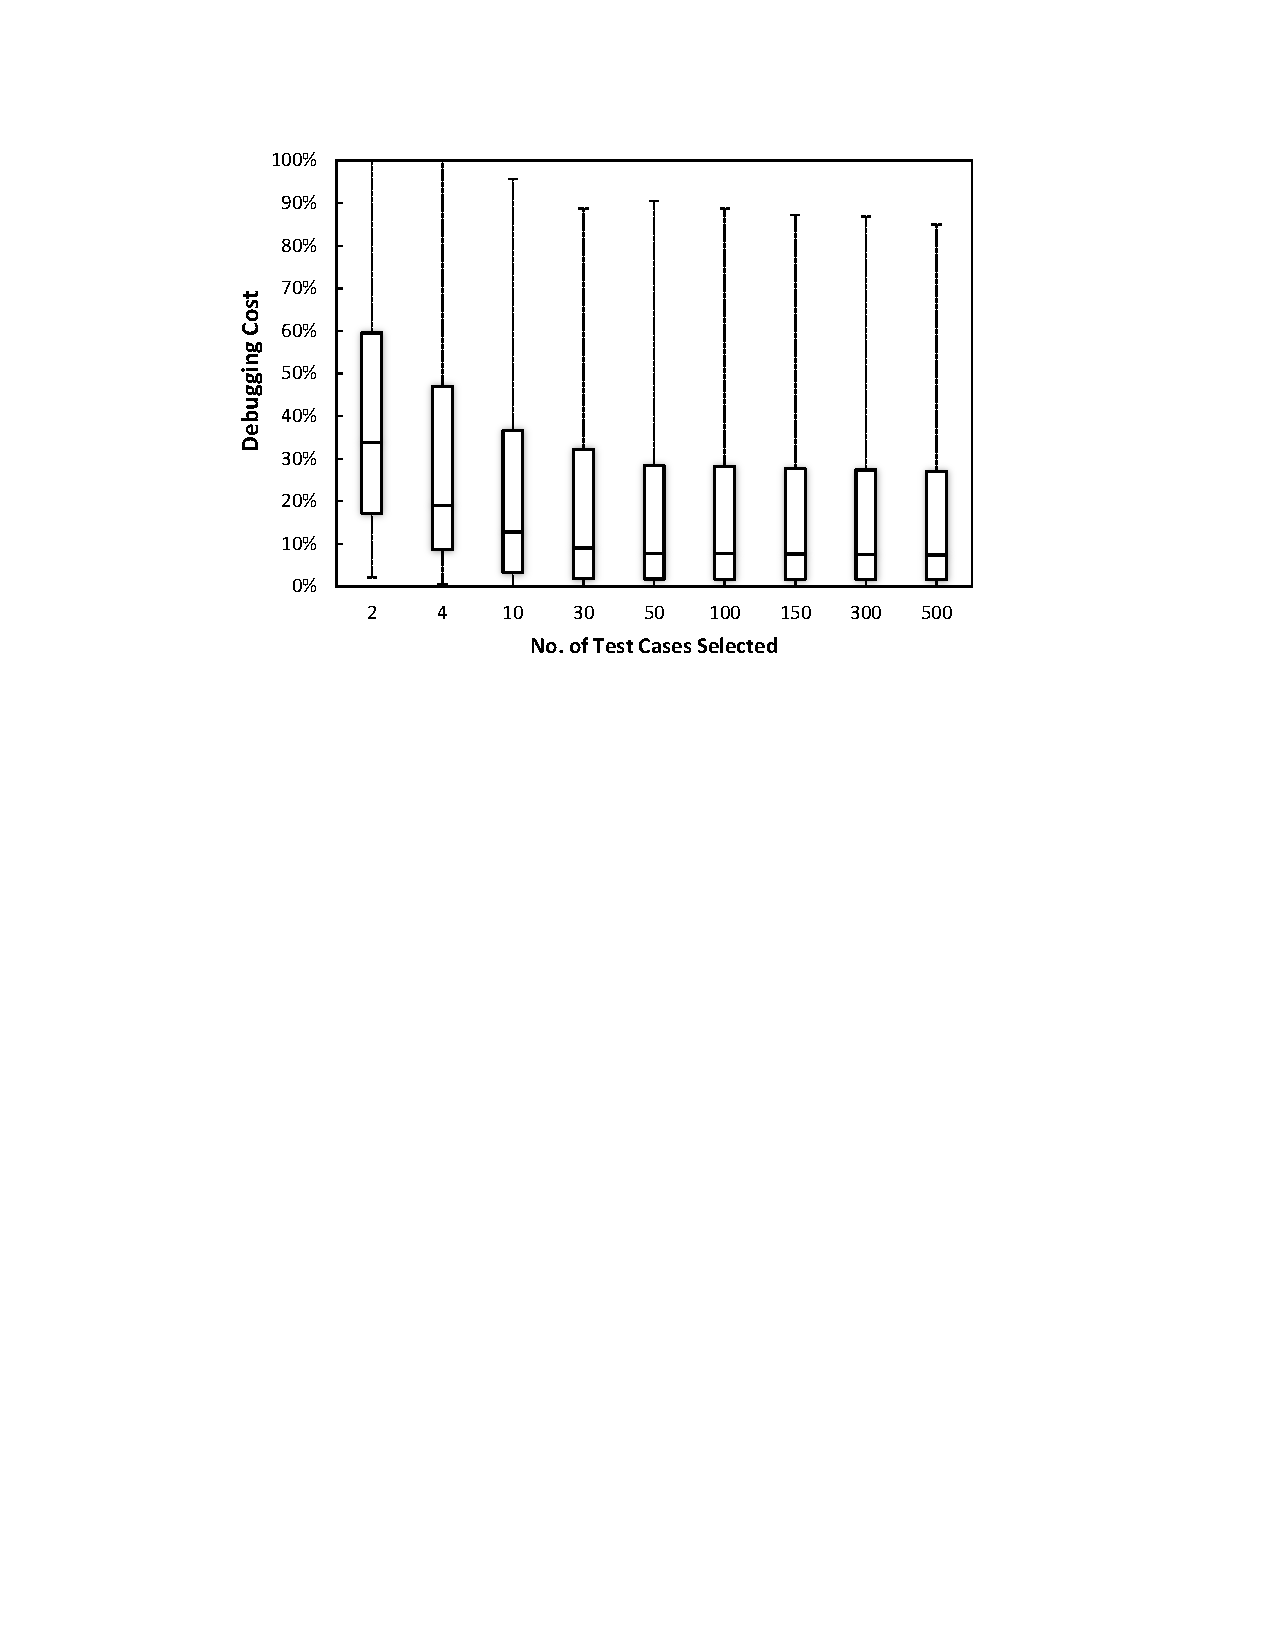
\includegraphics[width=12cm]{sdm_boxplot.pdf}
   % \vspace*{-12pt}
    \caption{Average Cost of {\sc Dms} when Selecting Different Numbers of Test Cases.}
    \label{Dms_boxplot}
\end{figure}

Following \cite{BaahPH10,BaahPH11} and the {\em cost}
metric (Equation~\ref{equation.avgcost}), we compare
the effectiveness of two prioritization methods $P_A$ and $P_B$ by using
one of the methods (for example, $P_B$) as reference measure.
When selecting the same number of traces $k$, the cost difference:
$cost(P_B) - cost(P_A)$ is considered as the improvement of $P_A$
over $P_B$. A positive value means that $P_A$ performs better than
$P_B$ (since lower cost is better) and a negative value means that the performance deteriorates if we use $P_A$ to replace $P_B$.
The difference corresponds
to the magnitude of improvement. For example, if the cost of
test cases from $P_A$ is 30\% and the cost of $P_B$ is 40\%,
then the improvement of $P_A$ over $P_B$ is 10\%, which means
that developers would examine 10\% fewer statements if $P_A$
is deployed.

\vspace{0.2cm}
\noindent{\bf Result Summary.} Table \ref{tab:compare_11}, \ref{tab:compare_21}, and \ref{tab:compare_31} compare
our method with the existing prioritizing techniques. The results show that
our method outperforms no worse than other methods for the majority of faulty program versions.

%\vspace{-0.1cm}
\begin{table}[tbp]
%	\vspace{-8pt}
    \centering
		\caption{Comparison of Prioritization methods.}
		\renewcommand{\arraystretch}{1.5}
		\small
        \begin{tabular}{|c|c|c|c|}
			\hline
			Test Prioritization Method  &  Positive  &  Negative  &   Neutral  \\
			\hline\hline
			\textsc{Dms} vs \textsc{Raptor} & {\bf 25.20\%} &    19.29\% &    55.51\% \\
			\hline
			\textsc{Dms} vs \textsc{Sequoia} & {\bf 33.46\%} &    19.69\% &    46.85\% \\
			\hline
			\textsc{Dms} vs \textsc{Stmt-Addtl} & {\bf 42.13\%} &    19.29\% &    38.58\% \\
			\hline
			\textsc{Dms} vs \textsc{Stmt-Total} & {\bf 62.99\%} &     7.87\% &    29.13\% \\
			\hline
			\textsc{Dms} vs \textsc{Fep-Addtl} & {\bf 40.16\%} &    20.08\% &    39.76\% \\
			\hline
			\textsc{Dms} vs \textsc{Art-Min} & {\bf 31.50\%} &    19.29\% &    49.21\% \\
			\hline
		\end{tabular}
    \label{tab:compare_11}
\end{table}

%\vspace{-0.1cm}
As illustrated in Table \ref{tab:compare_11}, \textsc{Dms} performs
better than \textsc{Raptor} on 25.20\% of the faulty versions, worse
on 19.29\% of the faulty versions, and shows no improvement
on 55.51\% of the faulty versions. The first row of
Table \ref{tab:compare_21} characterizes the degree of positive improvement of
\textsc{Dms} over \textsc{Raptor}. As the table indicates, half of the 25.20\%
faulty versions with positive improvement values have improvements
between 0.03\% and 3.93\%, and the other half
have improvements between 3.93\% and 77.42\%. The average
positive improvement of \textsc{Dms} over \textsc{Raptor} is 7.71\%.

%\vspace{-0.1cm}
\begin{table}[tbp]
    \centering
		\caption{Distribution of positive improvements.}
		\renewcommand{\arraystretch}{1.5}
		\small
        \begin{tabular}{|c|c|c|c|c|}
			\hline
			Test Pri. Tech.  &        Max &       Mean &     Median &        Min \\
			\hline\hline
			\textsc{Dms} vs \textsc{Raptor} & {\bf 77.42\%} &     7.71\% &     3.93\% &     0.03\% \\
			\hline
			\textsc{Dms} vs \textsc{Sequoia} & {\bf 66.67\%} &    14.38\% &     8.06\% &     0.23\% \\
			\hline
			\textsc{Dms} vs \textsc{Stmt-Addtl} & {\bf 72.87\%} &    14.68\% &     5.17\% &     0.03\% \\
			\hline
			\textsc{Dms} vs \textsc{Stmt-Total} & {\bf 94.97\%} &    27.68\% &    22.29\% &     0.03\% \\
			\hline
			\textsc{Dms} vs \textsc{Fep-Addtl} & {\bf 45.90\%} &    13.83\% &     6.35\% &     0.03\% \\
			\hline
			\textsc{Dms} vs \textsc{Art-Min} & {\bf 53.81\%} &     7.70\% &     3.23\% &     0.03\% \\
			\hline
		\end{tabular}
    \label{tab:compare_21}
\end{table}

Table \ref{tab:compare_31} characterizes the degree of negative deterioration of
\textsc{Dms} over other techniques. As the first row in the table indicates, for half of the 19.29\%
faulty versions, {\sc Dms} deteriorates 
% with positive improvement values have improvements
between 0.03\% and 0.60\% from \textsc{Raptor}, and for the other half,
%have improvements 
{\sc Dms} deteriorates between 0.60\% and 1.15\%. The average
percentage of negative deterioration of \textsc{Dms} over \textsc{Raptor} is 0.54\%.

\begin{table}[tbp]
    \centering
		\caption{Distribution of negative deterioration.}
		\renewcommand{\arraystretch}{1.5}
		\small
        \begin{tabular}{|c|c|c|c|c|}
			\hline
			Test Pri. Tech.  &        Max &       Mean &     Median &        Min \\
			\hline\hline
			\textsc{Dms} vs \textsc{Raptor} & {\bf 1.15\%} &     0.54\% &     0.60\% &     0.03\% \\
			\hline
			\textsc{Dms} vs \textsc{Sequoia} & {\bf 31.71\%} &    4.01\% &     1.33\% &     0.03\% \\
			\hline
			\textsc{Dms} vs \textsc{Stmt-Addtl} & {\bf 30.73\%} &    4.14\% &     1.52\% &     0.03\% \\
			\hline
			\textsc{Dms} vs \textsc{Stmt-Total} & {\bf 27.88\%} &    4.61\% &    2.64\% &     0.17\% \\
			\hline
			\textsc{Dms} vs \textsc{Fep-Addtl} & {\bf 24.70\%} &    5.06\% &     2.15\% &     0.03\% \\
			\hline
			\textsc{Dms} vs \textsc{Art-Min} & {\bf 22.41\%} &     4.11\% &     1.72\% &     0.03\% \\
			\hline
		\end{tabular}
    \label{tab:compare_31}
\end{table}


We conduct paired Wilcoxon signed-rank test to confirm the difference in performance between \textsc{Dms} and six existing prioritization techniques.
The statistical test result rejects the null hypothesis and suggests that the improvements of \textsc{Dms} over other existing techniques 
are statistically significant
%better than the existing best approach on \textsc{Unix} programs 
at 95\% confidence interval.

\vspace{0.2cm}
\noindent{\bf Detailed Comparison.} Table \ref{tab:label_effort} shows that \textsc{Raptor}, \textsc{Fep-Addtl} and \textsc{Art-Min} achieve 101\% of base line effectiveness with less than 500 test cases on subject programs.
Figure~\ref{fig:our_vs_fep}, \ref{fig:our_vs_artmin}, and~\ref{fig:our_vs_ag_unix}
show the comparison of fault localization costs between {\sc Dms} and the three different
prioritization techniques.
The horizontal axes represent the number of versions that
show differences in the Cost of
fault localization. The vertical axes represent the percentage
difference in Costs. If \textsc{Dms} is better than the reference
method, the area above zero-level line will be larger.

\vspace{0.2cm}
\noindent{\it D{\scriptsize MS} vs F{\scriptsize EP}-A{\scriptsize DDTL}.}
Previous studies~\citep{RUCH01,SEAGMGR01} show that \textsc{Fep-Addtl} is the most
promising prioritizing method for fault detection.
%However \textsc{Fep-Addtl} is not suitable for diagnostic prioritization,
%since it is initially proposed for regression testing, which assumes that
%tester have already get test oracles for each test case. But measuring
%{\em FEP} requires test oracles for all test cases which are absent in our problem.
%As a result, without test oracles {\em FEP} cannot evaluate the fault
%detection rate of each test case on program mutants.
%To circumvent this problem, Alberto \etal~\citep{Gonzalez-SanchezPAGG11} approximated {\em FEP}
Without test oracles, \textsc{Fep} can be estimated by $1 - ${\em False Negative Rate} (\textsc{Fnr})~\citep{Gonzalez-SanchezPAGG11}
\footnote{\textsc{Fnr} is the program passing rate when program element is the real fault and executed in test case. Usually when
\textsc{Fnr} is high, the fault is difficult to be detected by Spectrum-based
fault localization techniques.} which is also used in our study.
Figure \ref{fig:our_vs_fep} presents the comparison
between \textsc{Dms} and \textsc{Fep-Addtl} over all faulty versions that show performance differences.
\textsc{Fep-Addtl} is used as the reference prioritization technique.
The baseline represents the fault localization cost on program spectra prioritized
by \textsc{Fep-Addtl}. Each program version is a bar in this graph and we remove
versions from the graph that have no cost differences.
In the figure, the vertical axis represents the magnitude of
improvement of \textsc{Dms} over \textsc{Fep-Addtl}.
If the bar of a faulty version is above the
horizontal axis, that means on this version \textsc{Dms} performs
better than \textsc{Fep-Addtl} (positive improvement) and the bars
below the horizontal axis represent faulty versions for which
\textsc{Dms} performs worse than \textsc{Fep-Addtl}.

\begin{figure}[tbp]
    \centering
    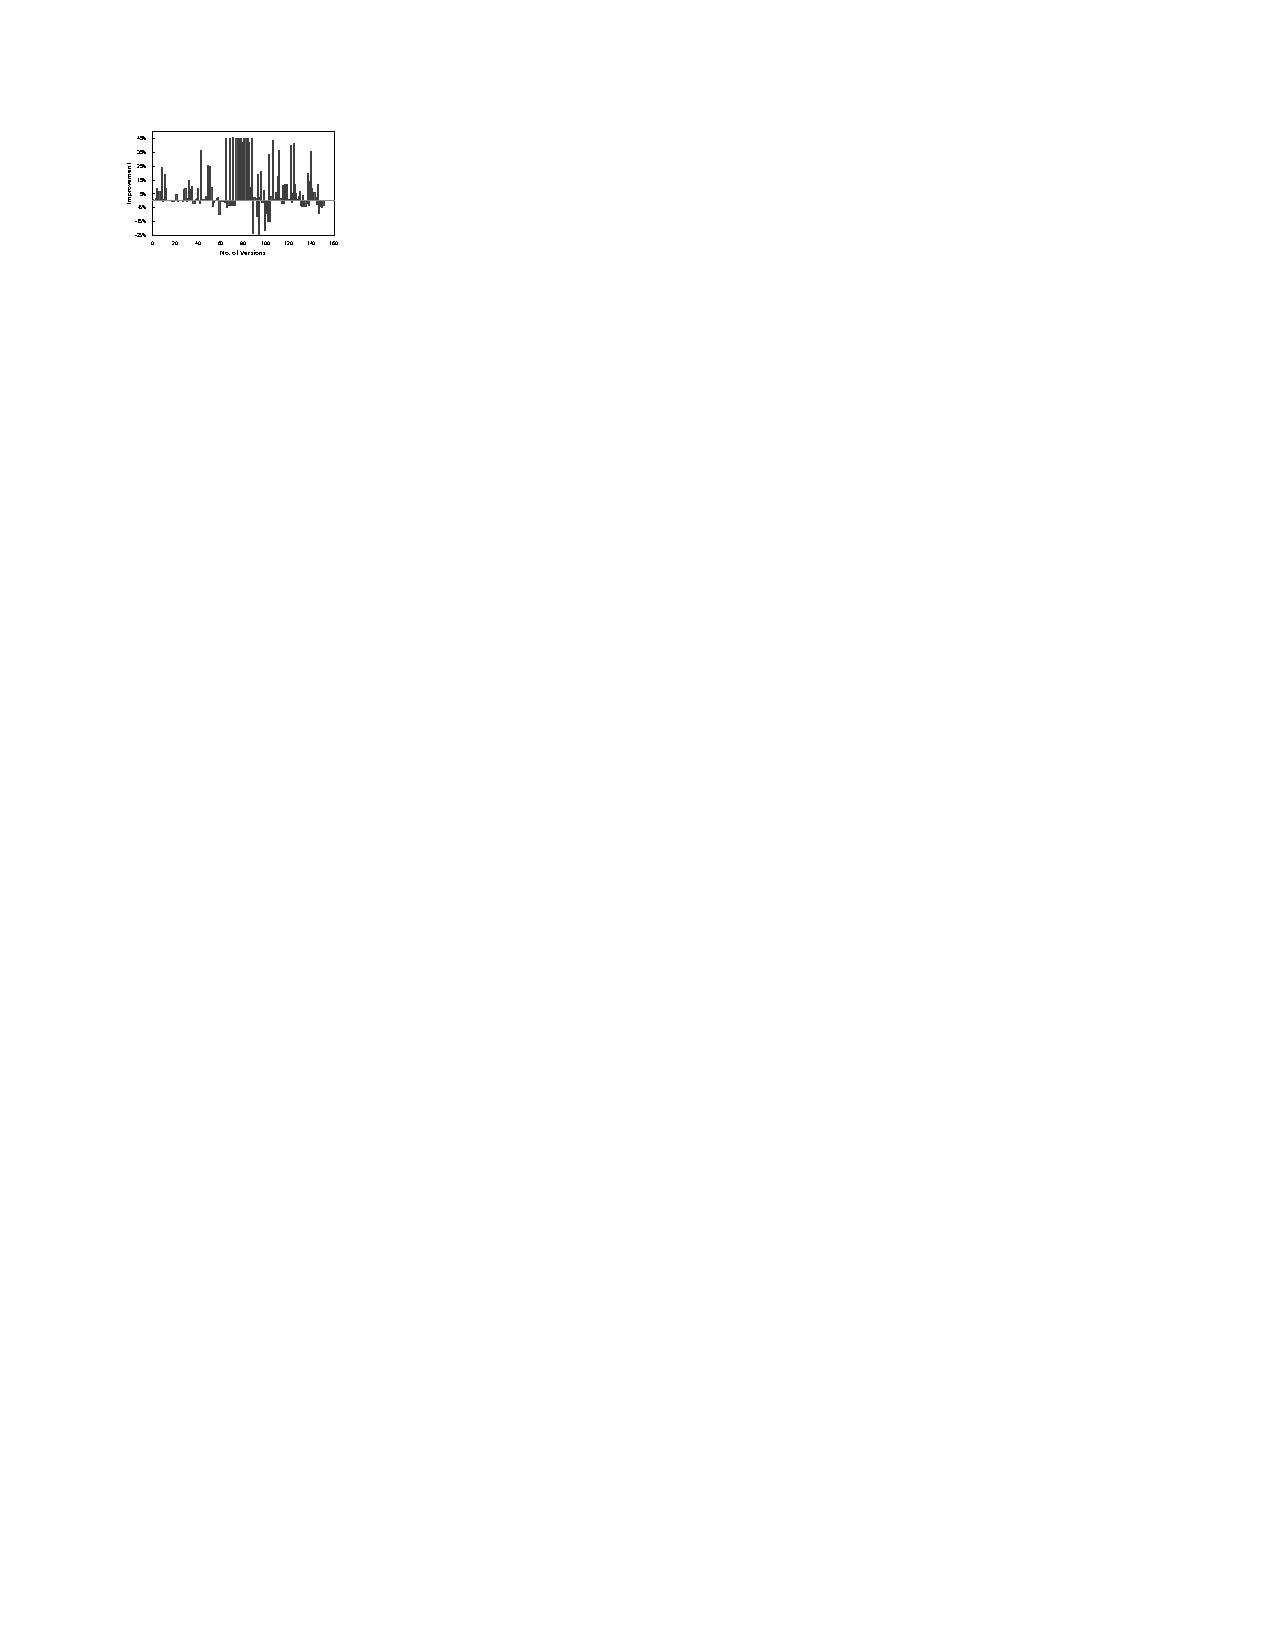
\includegraphics[width=12cm]{our_vs_fep.pdf}
%    \vspace{-0.3cm}
    \caption{Improvement of D{\scriptsize MS} over F{\scriptsize EP}-A{\scriptsize DDTL}.}
    \label{fig:our_vs_fep}
\end{figure}
%\vspace{0.2cm}

The comparison shows that \textsc{Dms} performs better than \textsc{Fep-Addtl} 
%for the majority of faulty versions.
%, our prioritization method performs
%better than \textsc{Fep-Addtl} 
on 102 versions, out of 153 versions that show differences in cost, but performs worse than
\textsc{Fep-Addtl} on 51 versions.
The positive improvement ranges from 0.03\% to 45.90\%, with an average of 6.35\%.


\begin{figure}[tbp]
    \centering
    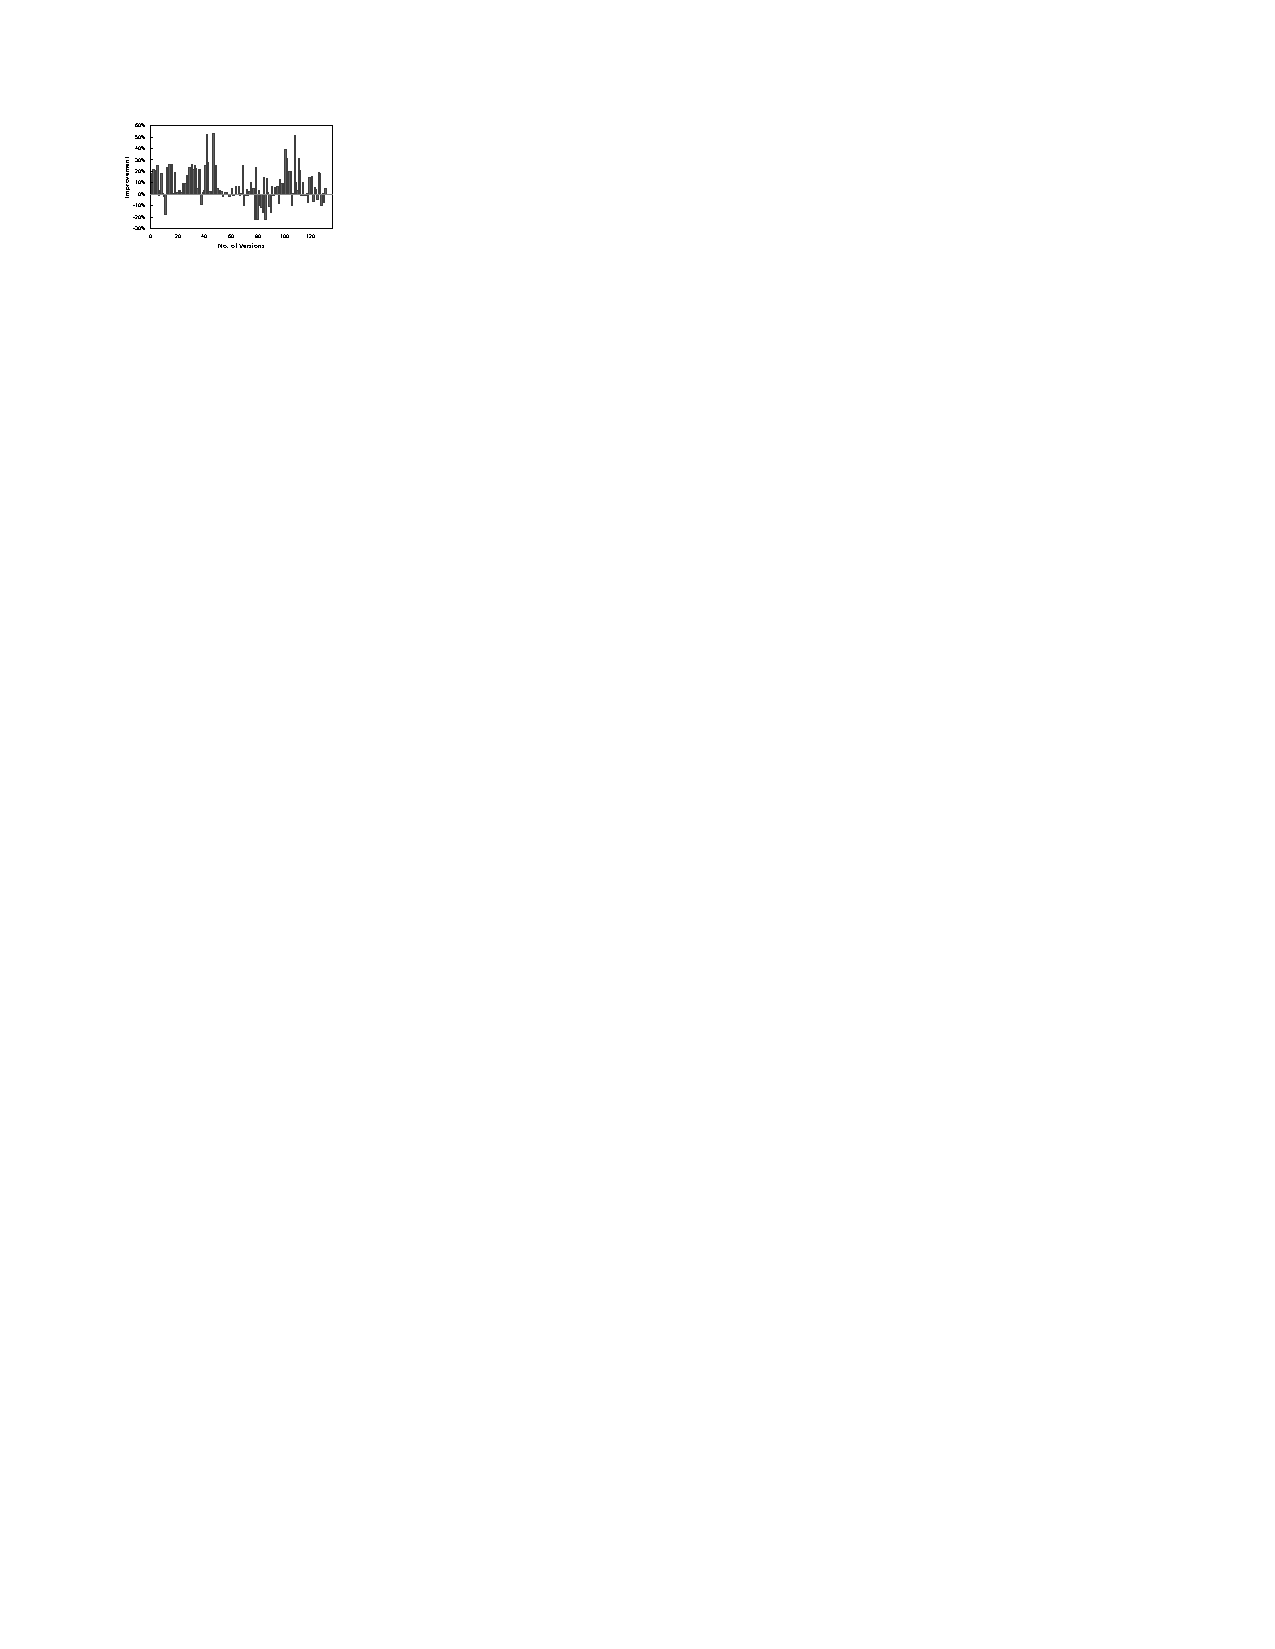
\includegraphics[width=12cm]{our_vs_artmin.pdf}
%    \vspace{-0.3cm}
    \caption{Improvement of D{\scriptsize MS} over A{\scriptsize rt}-M{\scriptsize IN}.}
    \label{fig:our_vs_artmin}
\end{figure}

\vspace{0.2cm}
\noindent{\it D{\scriptsize MS} vs A{\scriptsize rt}-M{\scriptsize IN}.} In this study we compare the effectiveness of \textsc{Dms} to {\em Adaptive Random Test Prioritization}(\textsc{Art})~\citep{JiangZCT09}.
There are various strategies for \textsc{Art}, in this experiment we only compare with the best one: \textsc{Art-Min}~\citep{JiangZCT09, Gonzalez-SanchezPAGG11, Alberto2011}.
Figure \ref{fig:our_vs_artmin} shows the results of the study in which \textsc{Art-Min} is used
as the baseline method. The comparison shows that \textsc{Dms} is better than \textsc{Art-Min}.
Out of 129 versions that show differences in cost, our prioritization method performs
better than \textsc{Art-Min} on 80 versions but performs worse than the
\textsc{Art-Min} on 49 versions.
%The positive improvement ranges from 0.03\% to 53.81\%, with an average of 7.70\%.

\vspace{0.2cm}
\noindent{\it D{\scriptsize MS} vs R{\scriptsize APTOR}.}
Figure \ref{fig:our_vs_ag_unix} shows the comparison between \textsc{Dms} and \textsc{Raptor} on \textsc{Unix} programs.
Here we use \textsc{Raptor} as the reference metric. The comparison shows that \textsc{Dms} 
%is better than \textsc{Raptor}.
%On \textsc{Unix} programs, 
outperforms \textsc{Raptor} on 20 versions by at least 1\% cost,
and on only 5 versions, it is worse than {\sc Raptor} by over 1\% cost.

\begin{figure}[tbp]
    \centering
    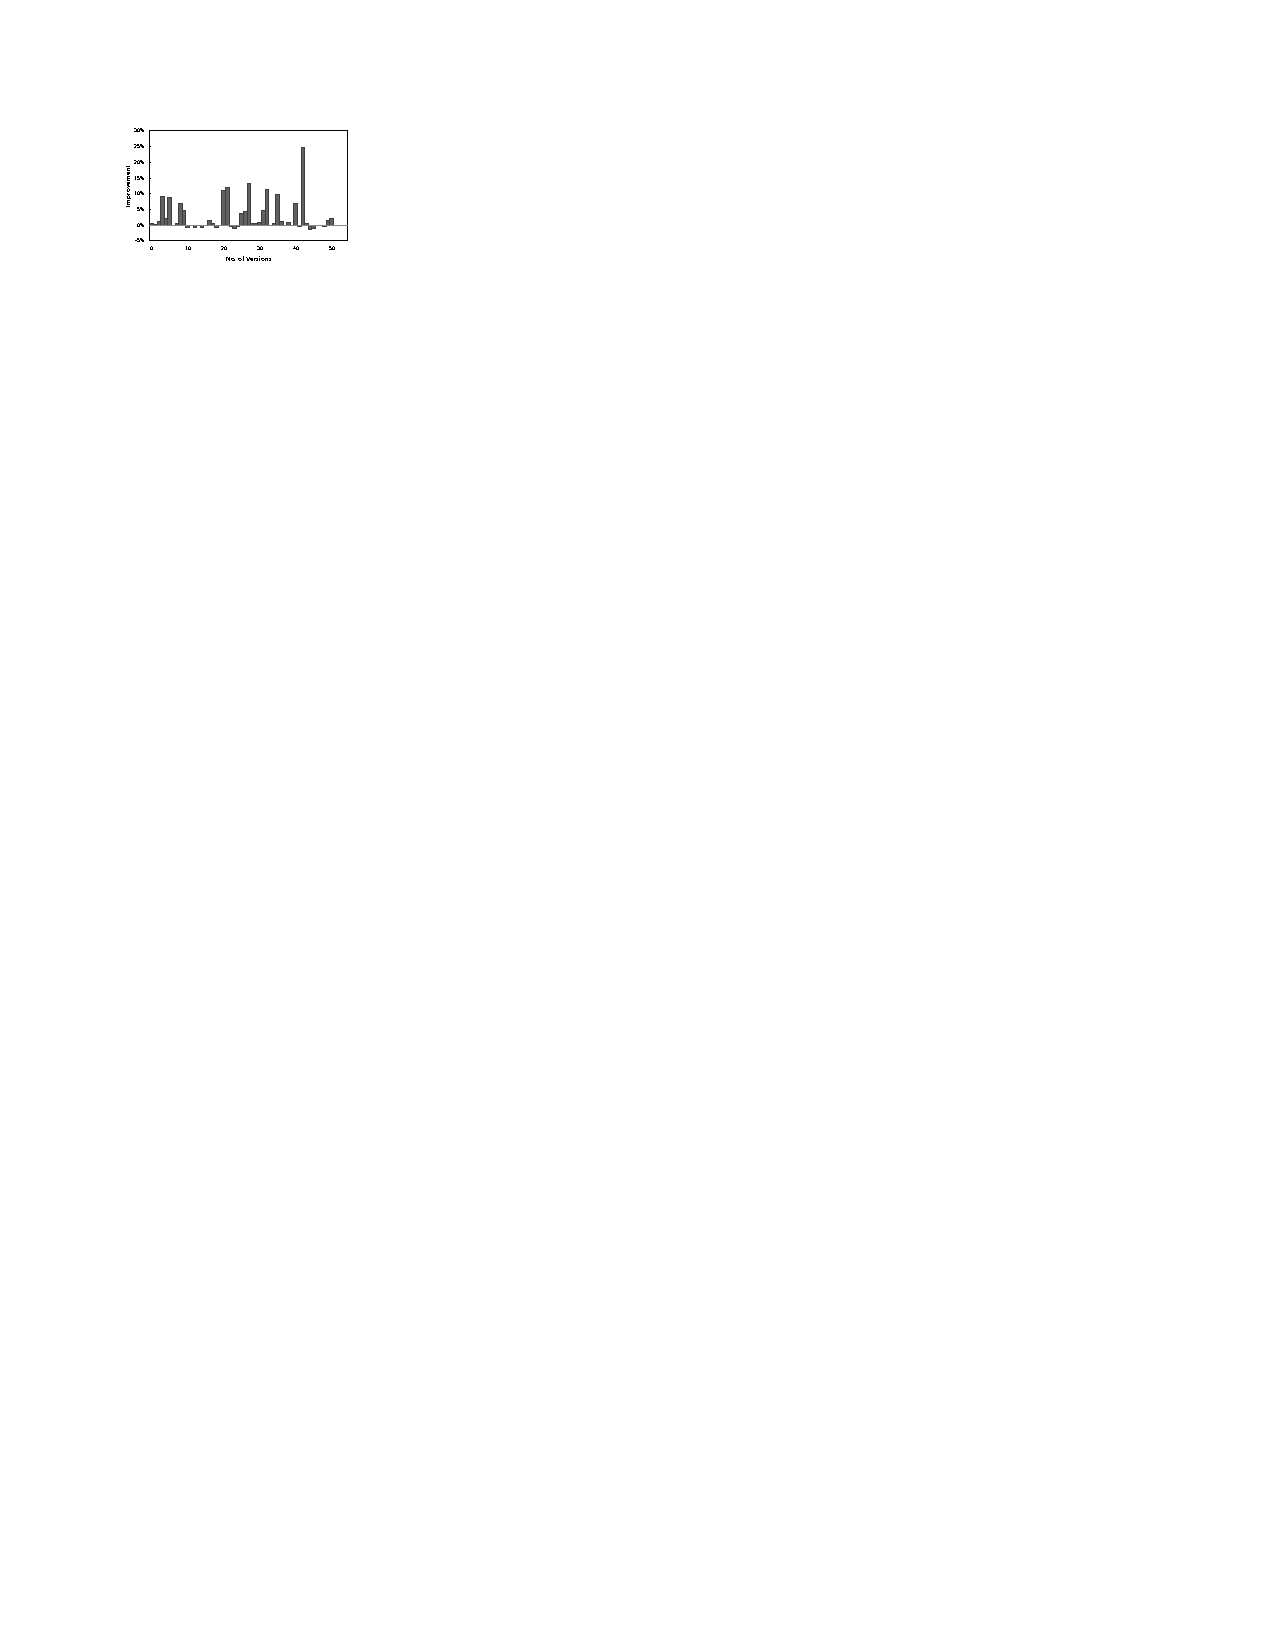
\includegraphics[width=12cm]{our_vs_ag_unix.pdf}
%    \vspace{-0.3cm}
    \caption{Improvement of D{\scriptsize MS} over R{\scriptsize APTOR} on U{\scriptsize NIX} programs.}
    \label{fig:our_vs_ag_unix}
\end{figure}

There is also improvement on Siemens programs: 32.2\% versions show differences and the average debugging cost improvement is 1.3\%, which is not so significant as compared with \textsc{Unix} programs.
This is probably due to the small software size. On Siemens programs, {\sc Raptor}
can reach 101\% of base line effectiveness by only selecting 20 test cases on average (see Table \ref{tab:label_effort}).
By selecting such few test cases, \textsc{Raptor} already obtains the maximal ambiguity group reduction due to very limited different
coverage profiles. For example, all test cases of \texttt{tcas} only have less than 15 ambiguity groups in all faulty versions. In this case,
the speedup by our method is trivial. In real scenario, programs to be diagnosed would be more similar to \textsc{Unix} programs.


\subsection{RQ2: multi-fault Programs}\label{sec.rq2}
Section~\ref{sec.exp.setup2} gives details about our experimental setup for multi-fault programs. Section~\ref{sec.exp.subject2} introduces the subject programs used in our study. Sections~\ref{sec.exp.resultsA2}~\&~\ref{sec.exp.resultsB2} show the results.

\subsubsection{Experimental Setups and Measures}\label{sec.exp.setup2}

The overall experimental setups and measures used for comparison for the multi-fault setting is similar to the single-fault setting. 

There is only a minor difference in the definition of the diagnostic cost as now there are multiple faults. The diagnostic cost is defined as follows:

\begin{equation}\label{equation.avgcost.multifault}
	cost = \dfrac{\left|  \left\{ j \left| \right.
           f_{T_{\mathcal{S}}}(d_j) \geq \min_{\substack{d_* \in D*}} f_{T_{\mathcal{S}}}(d_*) \right\} \right|}
           {\left|  \mathcal{D} \right|}
\end{equation}
where $\mathcal{D}$ consists of all program elements appearing in the program and $D_*$ is a set of faults in a program.
We calculate the average cost as the percentage of elements that developers have
to examine until locating all root causes ($D_*$). Since multiple
program elements can be assigned with the same suspiciousness score, the numerator
is considered as the number of program elements $d_j$ that have bigger or the
same suspiciousness score to a root cause $d_*$ in $D_*$ with the
lowest
%ambiguousness
suspiciousness
score. In this setting, we consider the worst-case scenario where developers need
to find all root causes by inspecting all elements that have a score no lower than the score of {\em any} root cause.

%In our experiment, every test case prioritization technique starts from an arbitrary labeled failed trace because developers start debugging only when test cases fail.

%We compare the effectiveness of different prioritization methods based on the diagnostic cost when the same number of test cases are selected.

%The diagnostic cost is defined as follows:
%\begin{equation}\label{equation.avgcost}
%	cost = \dfrac{\left|  \left\{ j \left| \right. f_{T_{\mathcal{S}}}(d_j) \geq f_{T_{\mathcal{S}}}(d_*) \right\}  \right|}{\left|  \mathcal{D} \right|}
%\end{equation}
%where $\mathcal{D}$ consists of all program elements appearing in the program.
%We calculate the average cost as the percentage of elements that developers have
%to examine until locating the root cause($d_*$) of failure. Since multiple
%program elements can be assigned with the same suspicious score, the numerator
%is considered as the number of program elements $d_j$ that have bigger or the
%same suspicious score to $d_*$.
%
%In this paper, we use \textsc{Raptor} as the bootstrapping technique ($\mathcal{P}$ in Figure \ref{algo:DMS}). During the bootstrapping process, $w$ is set to 10 to facilitate trend analysis.
%
%Following~\cite{JiangCT11}, for each faulty version, we repeat each prioritization technique 20 times to obtain its average cost. For each time, a randomly chosen failed trace is used as the starting point to alleviate the sensitivity of the technique to the choice of starting traces. On the other hand, to fairly compare our approach with other prioritization methods, the {\em same randomly} chosen failed traces are used as the starting traces for all methods.

\subsubsection{Subject Programs}\label{sec.exp.subject2}

Each multi-fault program version used in our study contains more than one fault where each fault involves only one line (or one simple statement if the statement is broken into more than one line) in the program and different faults affect different lines. This consideration is aligned with previous studies \citep[e.g.][]{zhang2013bridging,Abreu:2009.jss}. We use a dataset containing 173 multi-fault versions of 8 C programs as shown in Table~\ref{tab:multibug}. Different versions may contain the same fault, and there are 157 distinct faults in total. The dataset was previously used by \cite{lucia2013} to evaluate 40 different association measures.

%As print_token and schedule2 datasets only have four and seven bugs that involve one line, we randomly insert two bugs for every version, whereas for other datasets, we randomly insert five bugs for every multiple-bug version. Also, we ensure that each bug has been inserted at least in one of the versions. We generate multiple-bug versions for each dataset as many as the number of single-bug versions in the dataset. For example, there are 38 single-bug versions for Space, so we randomly generate 38 multiple-bug versions for Space, each of which contains five bugs. For each print_tokens and schedule2 dataset, we generate 10 multiple-bug versions. Thus, we have 20 multiple-bug versions that contain two bugs (minimum number of multiple bugs) and 153 versions that contain five bugs.

\begin{table}[!htbp]
	%\vspace{-8pt}
	\centering
	\caption{multi-fault Subject Programs}\label{tab:multibug}
	\renewcommand{\arraystretch}{1.5}
	%\small
    \begin{tabular}{|l|c|c|c|} \hline
        Program & \# Bugs Per Version &\# Tests& \# Versions\\ \hline\hline
		tcas & 5 &1,608& 41\\ \hline
        schedule2 & 2& 2,710 & 10\\ \hline
        schedule & 5&2,650 & 9\\ \hline
        replace & 5&5,542 & 32\\ \hline
		tot\_info & 5 &1,052 & 23\\ \hline
        print\_tokens2 & 5 &4,115& 10\\ \hline
        print\_tokens & 2&4,130 & 10\\ \hline
        space & 5&1,343 & 38\\ \hline
	\end{tabular}
\end{table}


%We use five real {\em C} programs and seven Siemens test programs from the {\em Software-artifact Infrastructure Repository}~(SIR)~\cite{doESE05}. We refer to the five real programs (\texttt{sed}, \texttt{flex}, \texttt{grep}, \texttt{gzip}, and \texttt{space}) as \textsc{Unix} programs. Table \ref{dataset} shows the descriptive statistics of each subject, including the number of faults, available test cases and code size. Following \cite{JHS02,Abreu:2009.jss}, we exclude faults not directly observable by the profiling tool\footnote{http://gcc.gnu.org/onlinedocs/gcc/Gcov.html} (e.g., some faults lead to a crash before \texttt{gcov} dumps profiling information and some faults do not cause any test case to fail), and in total we study 254 faults.


\subsubsection{Experimental Results: Reducing Number of Test Cases}\label{sec.exp.resultsA2}
%In this subsection, we conduct several controlled experiments to show the effectiveness of \textsc{Dms}.

%\vspace{-4pt}
%\subsubsubsection{Effectiveness on Reducing The Number of Test Cases Needed for a Target Cost}

We investigate the effectiveness of \textsc{DMS} in reducing the number of test cases needed for a targeted diagnostic cost for our multi-fault subject programs. Table \ref{tab:label_effort2} shows how many labels are needed on average to achieve 101\% of base line effectiveness (cf.\ Section \ref{sec.exp.setup}) for each approach. For example, \textsc{Raptor} requires 98 labels on average for each faulty version from all of the eight program datasets while \textsc{Dms} needs 79. In total, \textsc{Dms} requires the least amount of labeling effort; in comparison with the existing best approach (\textsc{FepAddtl}), \textsc{Dms} achieves 5.95\% labeling reduction on all of the datasets.

\begin{table}[!htbp]
%	\vspace{-8pt}
	\centering
	\caption{Labeling Effort on Subject Programs}
{
	\scriptsize
		\renewcommand{\arraystretch}{1.5}
		\hspace{-10pt}
        \begin{tabular}{|m{29pt}|m{13pt}|c|c|m{21pt}|m{21pt}|m{21pt}|m{17pt}|}
		   \hline
		     Subject &             &                &           & \textsc{Stmt-} & \textsc{Stmt-} & \textsc{Fep-}  & \textsc{Art-} \\
		   Programs & \textsc{Dms} & \textsc{Raptor}  & \textsc{Sequoia} & \textsc{Addtl} & \textsc{Total} & \textsc{Addtl} & \textsc{Min} \\
		   \hline\hline
		   All &   {\bf 79} &         98 &      111 &       102 &     240 &         84 &      164 \\
		   \hline
		 %  space &   {\bf 39} &         25&    72 &       48 &       305 &         71 &         73 \\
%		   \hline
		\end{tabular}
}
	\label{tab:label_effort2}
\end{table}


%\vspace{-6pt}
\subsubsection{Experimental Results: Reducing Cost}\label{sec.exp.resultsB2}
%\subsubsubsection{Effectiveness on Reducing Cost for a Given Number of Labeled Test Cases}

This subsection investigates the effectiveness of \textsc{Dms} in reducing cost given a targeted number of labeled test cases. Similar to the single-fault setting, we select 30 test cases and utilize the same method to compare between techniques. We also find that in our evaluation the average debugging cost of using \textsc{Dms} will not reduce significantly even if more labeled test cases than 50 are added further (see Figure \ref{fig:costmulti}).


\begin{figure}[tbp]
    \centering
    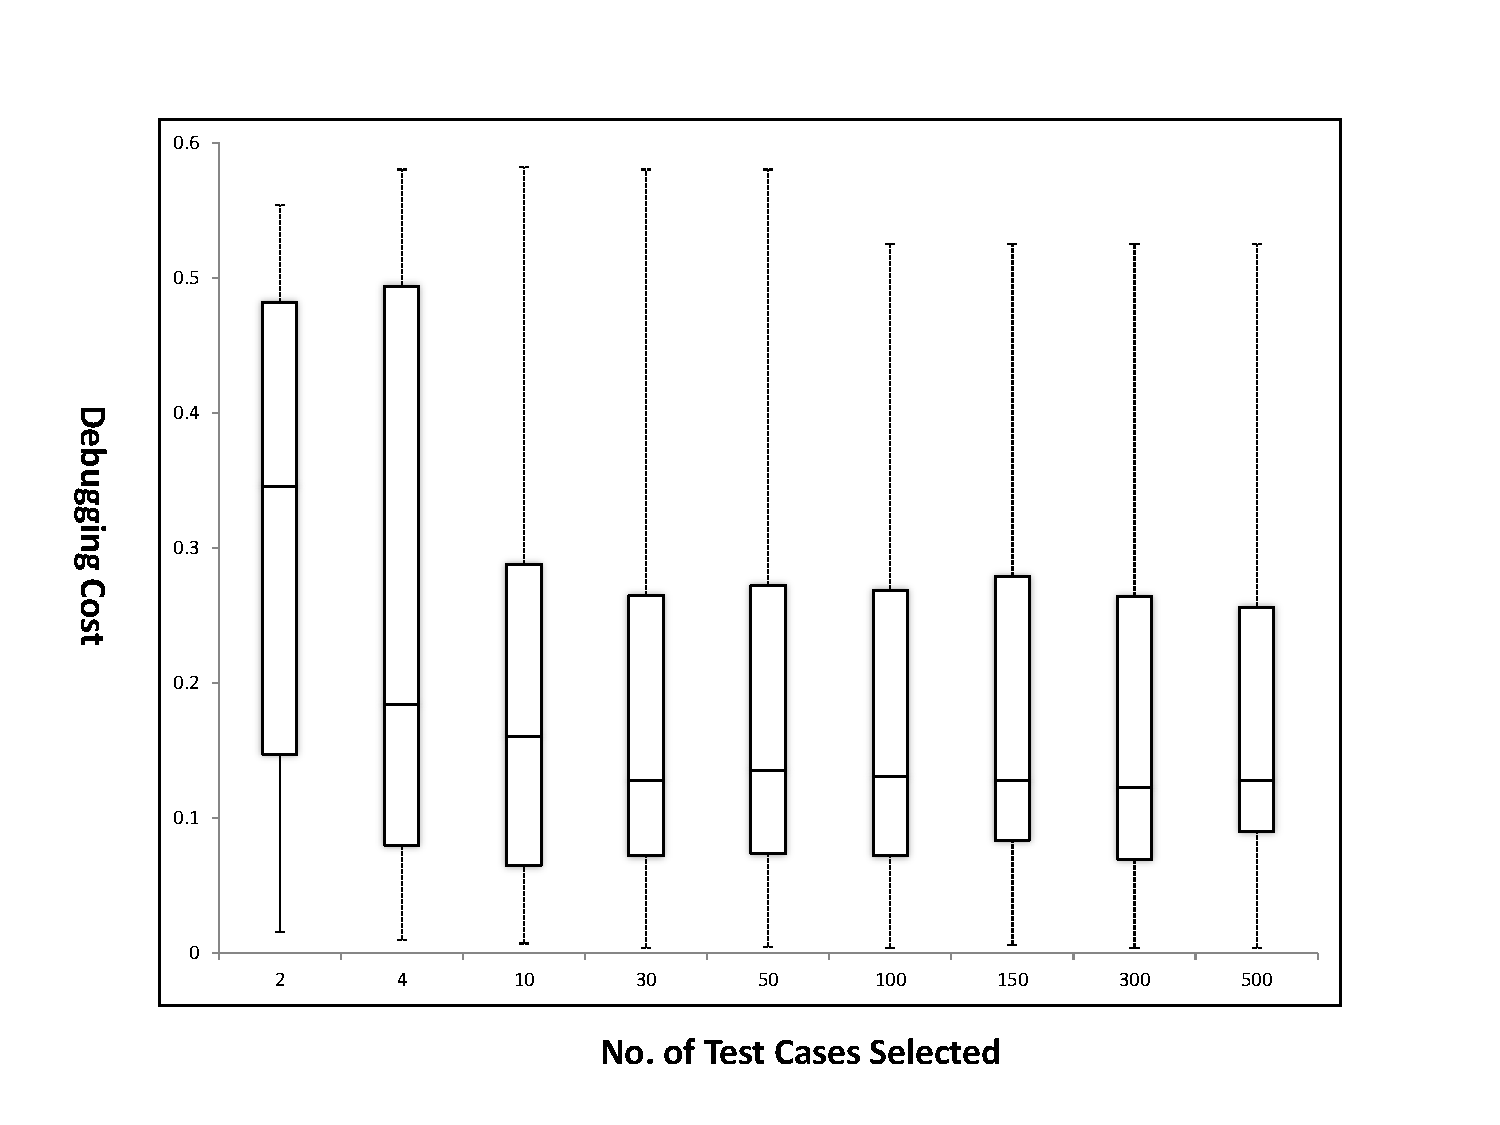
\includegraphics[width=12cm]{mut-sdm.pdf}
    %\vspace{-0.3cm}
    \caption{Average Cost of DMS when Selecting Different Numbers of Test Cases.}\label{fig:costmulti}

\end{figure}

\vspace{0.2cm}
\noindent{\bf Summary.} Table \ref{tab:compare_1}, \ref{tab:compare_2}, and~\ref{tab:compare_2_neg} summarize the comparison between our method and the existing prioritizing techniques.
%, the results show that our method outperforms all of them.
%\vspace{-0.1cm}
Table \ref{tab:compare_1} illustrates the distributions of {\sc Dms}'s performance against other techniques. For example, the first row shows that \textsc{Dms} performs better than \textsc{Raptor} on 34.68\% of the faulty versions, worse on 31.79\% of the faulty versions, and shows no improvement on 33.53\% of the faulty versions. The first row of Table~\ref{tab:compare_2} characterizes the degree of positive improvement of \textsc{Dms} over \textsc{Raptor}. As the table indicates, half of the 34.68\% faulty versions with positive improvement values have improvements between 0.03\% and 1.05\%, and the other half have improvements between 1.05\% and 46.75\%. The average positive improvement of \textsc{Dms} over \textsc{Raptor} is 5.95\%.
Table \ref{tab:compare_2_neg} illustrates the degree of negative deterioration of {\sc Dms} over other techniques. The first row shows that, half of the 31.79\% faulty versions for which {\sc Dms} performs worse than {\sc Raptor} have deterioration between 0.23\% and 2.94\%, and the other half have deterioration between 2.94\% and 53.30\%. The average deterioration of \textsc{Dms} from \textsc{Raptor} is 8.54\%.

\begin{table}[tbp]
%	\vspace{-8pt}
    \centering
		\caption{Comparison of Prioritization methods.}
		\renewcommand{\arraystretch}{1.5}
		\small
        \begin{tabular}{|c|c|c|c|}
			\hline
			Test Prioritization Method  &  Positive  &  Negative  &   Neutral  \\
			\hline\hline
			\textsc{Dms} vs \textsc{Raptor} & {\bf 34.68\%} &    31.79\% &    33.53\% \\
			\hline
			\textsc{Dms} vs \textsc{Sequoia} & {\bf 46.24\%} &    39.31\% &    14.45\% \\
			\hline
			\textsc{Dms} vs \textsc{Stmt-Addtl} & {\bf 50.29\%} &    28.23\% &    21.39\% \\
			\hline
			\textsc{Dms} vs \textsc{Stmt-Total} & {\bf 71.10\%} &    24.86\% &    4.05\% \\
			\hline
			\textsc{Dms} vs \textsc{Fep-Addtl} & {\bf 51.45\%} &   29.48\% &    19.08\% \\
			\hline
			\textsc{Dms} vs \textsc{Art-Min} & {\bf 71.68\%} &    23.70\% &    4.62\% \\
			\hline
		\end{tabular}
    \label{tab:compare_1}
\end{table}


\begin{table}[tbp]
    \centering
		\caption{Distribution of positive improvements.}
		\renewcommand{\arraystretch}{1.5}
		\small
        \begin{tabular}{|c|c|c|c|c|}
			\hline
			Test Prioritization Method  &        Max &       Mean &     Median &        Min \\
			\hline\hline
			\textsc{Dms} vs \textsc{Raptor} & {  46.75\%} &     5.95\% &     1.05\% &     0.03\% \\
			\hline
			\textsc{Dms} vs \textsc{Sequoia} & {  51.75\%} &   18.31\% &     14.31\% &     0.56\% \\
			\hline
			\textsc{Dms} vs \textsc{Stmt-Addtl} & {   54.24\%} &    10.67\% &     4.50\% &     0.04\% \\
			\hline
			\textsc{Dms} vs \textsc{Stmt-Total} & {  56.31\%} &    19.25\% &    25.42\% &     0.19\% \\
			\hline
			\textsc{Dms} vs \textsc{Fep-Addtl} & {  99.05\%} &    17.94\% &     9.04\% &     0.02\% \\
			\hline
			\textsc{Dms} vs \textsc{Art-Min} & {  99.13\%} &     42.96\% &     36.83\% &     0.14\% \\
			\hline
		\end{tabular}
    \label{tab:compare_2}
\end{table}


\begin{table}[tbp]
    \centering
		\caption{Distribution of negative deterioration.}
		\renewcommand{\arraystretch}{1.5}
		\small
        \begin{tabular}{|c|c|c|c|c|}
			\hline
			Test Prioritization Method  &        Max &       Mean &     Median &        Min \\
			\hline\hline
			\textsc{Dms} vs \textsc{Raptor} & {  53.30\%} &     8.54\% &     2.94\% &     0.23\% \\
			\hline
			\textsc{Dms} vs \textsc{Sequoia} & {  52.00\%} &   8.49\% &     4.37\% &     0.19\% \\
			\hline
			\textsc{Dms} vs \textsc{Stmt-Addtl} & {  53.86\%} &    10.88\% &     4.87\% &     0.14\% \\
			\hline
			\textsc{Dms} vs \textsc{Stmt-Total} & { 51.38\%} &   10.56\% &   7.10\% &     0.13\% \\
			\hline
			\textsc{Dms} vs \textsc{Fep-Addtl} & {  47.13\%} &    10.72\% &     5.89\% &     0.04\% \\
			\hline
			\textsc{Dms} vs \textsc{Art-Min} & {  46.21\%} &     3.33\% &     2.01\% &     0.16\% \\
			\hline
		\end{tabular}
    \label{tab:compare_2_neg}
\end{table}

We conduct paired Wilcoxon signed-rank test to confirm the difference in performance between \textsc{Dms} and six existing prioritization techniques. The statistical test result rejects the null hypothesis and suggests that the performance differences between \textsc{Dms} and other techniques are statistically significant
%ly better than the existing best approach on the multi-fault subject programs 
at 95\% confidence interval.

\vspace{0.2cm}\noindent{\bf Detailed Comparison.}
Similar to the single-fault setting, 
%Table \ref{tab:label_effort} shows that \textsc{Raptor}, \textsc{Fep-Addtl} and \textsc{Art-Min} achieve 101\% base line effectiveness with less than 500 test cases on subject programs. We only 
we show the comparison between \textsc{Dms} and three methods, \textsc{Raptor}, \textsc{Fep-Addtl} and \textsc{Art-Min}, in terms of fault localization costs in Figure~\ref{fig:our_vs_fep.multifault}, \ref{fig:our_vs_artmin.multifault}, and~\ref{fig:our_vs_raptor.multifault}.
%show the comparison between different prioritization techniques based on fault localization cost.

\vspace{0.2cm}\noindent{\it D{\scriptsize MS} vs F{\scriptsize EP}-A{\scriptsize DDTL}.}
Figure \ref{fig:our_vs_fep.multifault} presents the comparison between \textsc{Dms} and \textsc{Fep-Addtl} over all faulty versions that show cost differences. The comparison shows that \textsc{Dms} is better than \textsc{Fep-Addtl} on 89 versions, out of 140 versions that show differences in cost, 
but performs worse than the \textsc{Fep-Addtl} on 51 versions. The positive improvement ranges from 0.02\% to 99.05\%, with an average of 17.94\%.

%Previous studies~\cite{RUCH01,SEAGMGR01} show that \textsc{Fep-Addtl} is the most promising prioritizing method for fault detection.
%However \textsc{Fep-Addtl} is not suitable for diagnostic prioritization,
%since it is initially proposed for regression testing, which assumes that
%tester have already get test oracles for each test case. But measuring
%{\em FEP} requires test oracles for all test cases which are absent in our problem.
%As a result, without test oracles {\em FEP} cannot evaluate the fault
%detection rate of each test case on program mutants.
%To circumvent this problem, Alberto \etal~\cite{Gonzalez-SanchezPAGG11} approximated {\em FEP}
%Without test oracles, \textsc{Fep} can be estimated by $1 - ${\em False Negative Rate} (\textsc{Fnr})~\cite{Gonzalez-SanchezPAGG11}
%\footnote{\textsc{Fnr} is the program passing rate when program element is the real fault and executed in test case. Usually when
%\textsc{Fnr} is high, the fault is difficult to be detected by Spectrum-based
%fault localization techniques.} which is also used in our study.

%\vspace{0.2cm}
\vspace{0.2cm}\noindent{\it D{\scriptsize MS} vs A{\scriptsize rt}-M{\scriptsize IN}.}
We compare the effectiveness of \textsc{Dms} to the best variant of {\em Adaptive Random Test Prioritization}(\textsc{Art}), namely \textsc{Art-Min}~\citep{JiangZCT09, Gonzalez-SanchezPAGG11, Alberto2011}. Figure \ref{fig:our_vs_artmin.multifault} shows the results of the study in which \textsc{Art-Min} is used as the baseline method. The comparison shows that \textsc{Dms} is better than \textsc{Art-Min} on 124 versions, out of 165 versions that show differences in cost, 
but performs worse than the \textsc{Art-Min} on 41 versions.

%The positive improvement ranges from 0.03\% to 53.81\%, with an average of 7.70\%.

\vspace{0.2cm}\noindent{\it D{\scriptsize MS} vs R{\scriptsize APTOR}.}
Figure \ref{fig:our_vs_raptor.multifault} shows the comparison between \textsc{Dms} and \textsc{Raptor}. The comparison shows that \textsc{Dms} is better than \textsc{Raptor} on 60 versions, out of 115 versions that show differences in cost, 
but performs worse than the \textsc{Raptor} on 55 versions.
The average deterioration (8.54\%) of {\sc Dms} (Table \ref{tab:compare_2_neg} is higher than its average improvement (5.95\%) in comparison with {\sc Raptor} (Table \ref{tab:compare_2}), even though {\sc Dms} reduces the total labelling effort from 98 test cases to 79 (Table \ref{tab:label_effort2}). We are yet unclear about the reason causing the trade-off in the multi-fault programs. It is very intriguing future work to find ways to balance between labelling effort and diagnostic cost better.

%\textsc{Dms} outperforms \textsc{Raptor} on 20 versions by at least 1\% cost, and only 5 versions worse than \textsc{Raptor} over 1\% cost.

\begin{figure}[tbp]
    \centering
    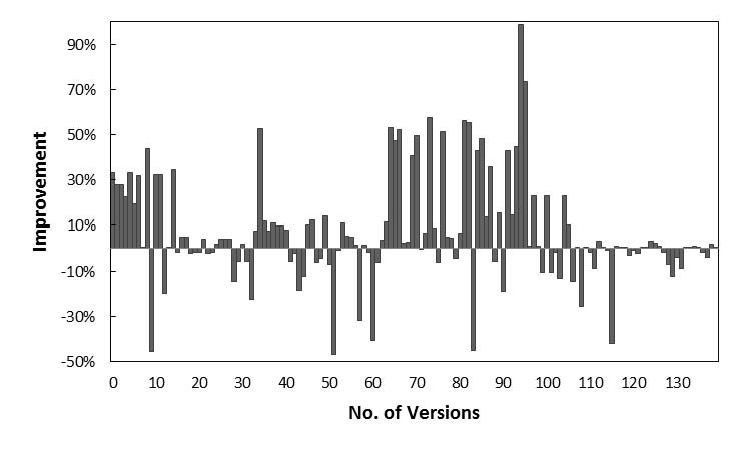
\includegraphics[width=12cm]{mut-dms-feq.pdf}
%    \vspace{-0.3cm}
\caption{Improvement of D{\scriptsize MS} over F{\scriptsize EP}-A{\scriptsize DDTL}.}
    \label{fig:our_vs_fep.multifault}
\end{figure}
%\vspace{0.2cm}



\begin{figure}[tbp]
    \centering
    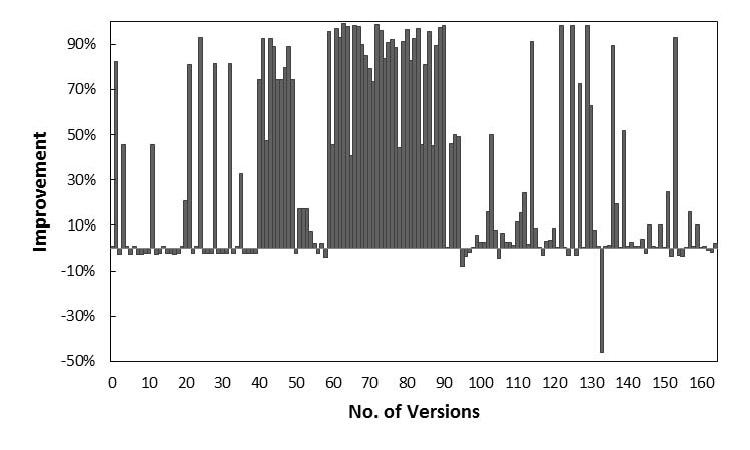
\includegraphics[width=12cm]{mut-dms-art.pdf}
%    \vspace{-0.3cm}
    \caption{Improvement of D{\scriptsize MS} over A{\scriptsize rt}-M{\scriptsize IN}.}
    \label{fig:our_vs_artmin.multifault}
\end{figure}

\begin{figure}[tbp]
    \centering
    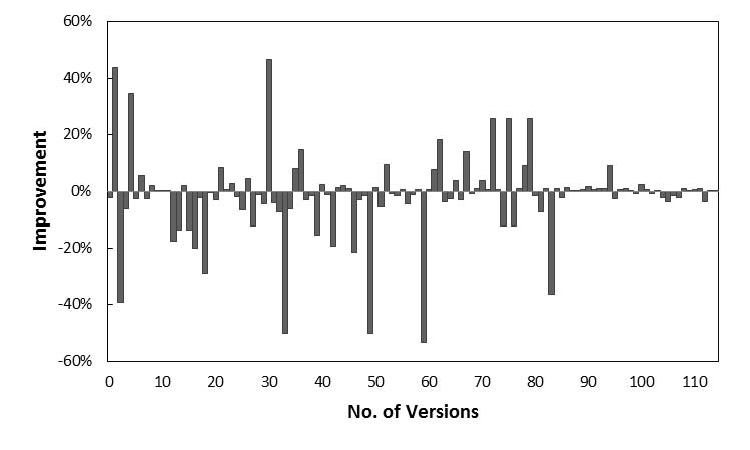
\includegraphics[width=12cm]{mut-dms-raptor.pdf}
%    \vspace{-0.3cm}
\caption{Improvement of D{\scriptsize MS} over R{\scriptsize APTOR}.}
    \label{fig:our_vs_raptor.multifault}
\end{figure}

%on U{\scriptsize NIX} programs

%There is also improvement on Siemens programs: 32.2\% versions show differences and the average debugging cost improvement is 1.3\%, which is not so significant as comparison on \textsc{Unix} programs.
%This is probably due to the small software size. On Siemens programs the existing best approach
%can reach 101\% of the base line effectiveness by only selecting less than 20 test cases on average (see Table \ref{tab:label_effort}).
%By selecting such few test cases, \textsc{Raptor} already obtains the maximal ambiguity group reduction due to very limited different
%coverage profiles. For example, all test cases of \texttt{tcas} only have less than 15 ambiguity groups in all faulty versions. In this case,
%the speedup by our method is trivial. In real scenario, programs to be diagnosed would be more similar to \textsc{Unix} programs.


\subsection{Discussion and Threats to Validity}\label{sec.exp.threats}
As we noticed, the improvement of \textsc{Dms} in single-fault and multi-fault programs are different. In the 12 single-fault programs,  \textsc{Dms} requires the minimal amount of labeling effort by achieving 67.7\% labeling reduction on Unix programs and 10\% reduction on Siemens programs in comparison with the existing best approach---Raptor. While in the 8 multi-fault programs, \textsc{Dms} achieves 5.95\% labeling reduction in comparison with the existing best approach---Fep-Addtl. The phenomenon happens since we consider the worst cases of \textsc{Dms} in multi-fault programs, i.e., we consider the root case $d_*$ with the lowest suspiciousness score. In some versions of the multi-fault programs, \textsc{Dms} needs more test cases to achieve the value of $c_x$ than that of Fep-Addtl. For example, in the version 2 of the program print\_token2, \textsc{Dms} need to label 500 test cases to achieve $c_x$, while Fep-Addtl only requires 59 test cases. Thus, the reduced number of test cases for \textsc{Dms} in multi-fault program is not as high as that in single-fault program.

However, the improvement of \textsc{Dms} in reducing cost is significant for both single-fault and multi-fault programs. The statistics of  paired Wilcoxon signed-rank test show that \textsc{Dms} is statistically significantly better than the existing best approach on the Unix programs of single-fault subject programs, and multi-fault subject programs at 95\% confidence interval. Moreover, although we notice that \textsc{Dms} reduce the number of test case of Fep-Addtl by 5.95\% in multi-fault programs, but there are 51.45\% fault versions that \textsc{Dms} show positive improvement over Fep-Addtl, and  29.48\% fault versions that \textsc{Dms} show negative improvement over Fep-Addtl, while the number for single-fault programs are 40.16\% and 20.08\%.


The threats to our studies include the issue of how
representative the subjects of our studies are. Since the Siemens programs
are small and larger programs may be subject to different testing and debugging traits.
To strengthen the external validity, we include \textsc{Unix} programs which are
real-life programs. These subjects have been adopted for evaluation in many
studies \citep[e.g.][]{JH05,Abreu:2009.jss,DBLP:conf/icse/SantelicesJYH09}.

Another possible threat is that although our method outperforms existing method
in 25.2\% to 62.99\% program versions and gets equivalent cost in around 30\% versions,
there are still a certain percent of versions that our method does not perform very well.
But as we can see in the studies, most of the negative improvements of those versions
are relatively small or even trivial comparing to the positive improvements. We also
conduct statistical test to further confirm the superiority of \textsc{Dms}.

%At last, the studies show that \textsc{Dms} outperforms other methods
%in reducing manual effort for debugging, but the ultimate
%merit should be evaluated by end-users. However, due to the
%expense as well as difficulty of user study, most existing works in
%test case prioritization and fault localization are temporarily evaluated
%by authors~\cite{RUCH01,SEAGMGR01,LHH07,Abreu:2009.jss}.



%\vspace{-4pt}
\section{Related Work}\label{sec.related}
In this section, we describe related work on fault localization, defect prediction, test case prioritization,  diagnostic prioritization, and automated oracle construction. The survey here is by no means a complete list.



\smallskip\noindent
\textbf{Fault} \textbf{Localization.} Over the past decade, many automatic fault localization and debugging methods have been proposed.
The ways of calculating ambiguousness  for program elements are various, including state-of-arts (e.g. {\em Tarantula}~\citep{JHS02,JH05} and {\em Ochiai}~\citep{Abreu:2009.jss}).
%In recent work, Baah \etal propose using Probabilistic Program Dependence Graphl~\citep{BaahPH08} and
%causal inference~\citep{BaahPH10} that combines static dependency information and dynamic coverage information to diagnose the program.
%Their methods show a great improvement over contentional fault localization methods.
\cite{RR03} propose a nearest neighbor fault localization tool called \textsc{Whither} that compares the failed execution
to the correct execution and reports the most ambiguity  locations in the program.
\cite{Zeller2002a} applies {\em Delta Debugging} to search for the minimum state differences between a failed execution and a successful execution that may cause the failure. \cite{LAZJ03} consider predicates whose true evaluation correlates with failures are more likely to be the root cause. Campos et al. propose ENTBUG which applies entropy theory to guide test case generation~\cite{campos2013entropy}.
%Based on the similar intuition, \textsc{Sober}~\citep{LYFHM05} extends Liblit's method by incorporating information on the outcomes of multiple predicate evaluations and use statistical test to determine the difference between predicate values in passed and failed traces.

%Artzi \etal propose a directed test generation technique to provide enough test cases for fault localization techniques~\citep{ArtziDTP10,ADTP10b}. It is very effective for HTML pages since they are of rich structures. However, the code responsible for producing incorrect output might be the entire program, their method is unlikely to be effective for a program that produces simple structures or a single number.

%\noindent
%\textbf{Defect} \textbf{Prediction}
%In defect prediction, many works~\citep{Nagappan:2006:MMP:1134285.1134349,DBLP:conf/icsm/ZhangW10,DBLP:journals/ase/LiZWZ12} use software size, complexity metrics, and %variations of various variables in software development process to build prediction models. For example, Nagappan \etal~\citep{Nagappan:2006:MMP:1134285.1134349} %propose regression models with principal component analysis on the code metrics to predict post-release defects.
%In \citep{DBLP:conf/icsm/ZhangW10}, Zhang \etal construct defect prediction models based on a small number of randomly sampled program files. In \citep{DBLP:journals/ase/LiZWZ12}, they further propose an active learning based method for building defect prediction models.

%Some studies consider code structure to improve the prediction accuracy. e.g.,
%Shin~\etal use a fault model with information about call relations, which provided noticeable accuracy improvements over models without call information ~\citep{10.1109/MSR.2009.5069481}. In  \citep{Zimmermann:2008:PDU:1368088.1368161} network analysis is applied to identify defects.


%Model-based debugging techniques, e.g., \citep{Mayer2007,Feldman2006}, are relatively heavyweight and consider semantics of the code since they are based on expensive logic reasoning over formal models of programs. There are also other static and dynamic analysis techniques, e.g., \citep{fse:msady04,TTG08}, that are related to model-based debugging.
%Although few model-based techniques have employed the concept of failure association, incorporating association measures and other statistical analyses into program models can be a future direction for improving the performance of model-based debugging techniques.


\smallskip\noindent
\textbf{Test} \textbf{Case} \textbf{Prioritization.}
Test case prioritization techniques are initially proposed for early fault detection in regression testing. \cite{RUCH01} show the coverage-based and Fault-exposing-potential based approaches can improve the rate of fault detection of test suites. \cite{SEAGMGR01} further investigate ``version-specific prioritization" on different profile granularities. \citep{LHH07} show that {\em Additional Greedy Algorithm} is among the best approaches for regression test case prioritization.
%In \citep{Gonzalez-SanchezPAGG11}, Gonz{\'a}lez-Sanchez \etal adopt {\em information gain} for diagnostic prioritization.
\cite{DBLP:conf/icse/BaudryFT06} propose {\em Dynamic Basic Block} (\textsc{Dbb}) for test suite reduction. Their method focuses on the number of \textsc{Dbb}s.
\cite{Alberto2011} further consider group sizes for test suite reduction.

%Jiang \etal~\citep{JiangCT11} investigate various prioritization techniques and show that existing test adequacy criteria are still insufficient in supporting effective fault localization.

\smallskip\noindent
\textbf{Oracle} \textbf{Construction.}
Although in recent years, many studies \cite[e.g.][]{CPacheco05,Xie06,BRH04} aim to automatically generate test oracles, they are often heavy weight, based on certain assumption and thus applicable to specific scenarios. {\em Eclat} \citep{CPacheco05} can generate assertions based on a learning model, but they assume correct executions.
%In \citep{CPacheco07}, {\em Randoop} allows annotation of the source code to identify observer methods to be used for assertion generation.
\cite{Xie06} proposes a method called {\em Orstra} for oracle checking.
%{\em Orstra} generates assertions based on observed return values and object states and adds assertions to check future runs against these observations.
\cite{BRH04} propose \textsc{Argo} which selects test cases inducing unknown behaviors to actively construct test oracles for improving test quality. The approach is more suitable for regression testing. Our approach complements these studies by reducing the effort needed for the purpose of fault localization.



%\vspace{-4pt}
\section{Conclusion and Future Work} \label{sec.conclusion}
This paper proposes a new concept and technique named {\em Diversity Maximization Speedup} ({\sc Dms}) aiming to minimize the amount of effort in manual oracle construction, while still permitting effective fault localization. In comparison with six other existing prioritization techniques on 12 {\em C} programs, we have shown that our technique requires on average a smaller number of labelled test cases to achieve the targeted diagnostic cost of subsequent fault localization techniques, and that if the same number of labelled test cases are allowed, it can choose test cases that may be more effective in reducing debugging cost. We have shown that the improvements made by our technique on real-life programs over other existing techniques are statistically significant.

In future, we will evaluate the proposed approach on more subject programs. We will also explore the possibility of adopting more sophisticated trend analysis methods.

%Future work includes evaluation on more subject programs and further extension on our prioritization approach by adopting more sophisticated trend analysis methods.

%\vspace{-4pt}
\section{Acknowledgement} \label{sec.acknowledgement}
%\smallskip\noindent{\bf Acknowledgement.}
This work is partially supported by NSFC Program (No.61073006 and 61103032), Tsinghua University project 2010THZ0, and National Key Technology R\&D Program of the Ministry of Science and Technology of China (No2013BAH01B03). We thank researchers at University of Nebraska--Lincoln, Georgia Tech, and Siemens Corporate Research for the Software-artifact Infrastructure Repository. We would also like to thank the anonymous reviewers for providing us with constructive comments and suggestions.
 

%\begin{acknowledgements}
%If you'd like to thank anyone, place your comments here
%and remove the percent signs.
%\end{acknowledgements}

% BibTeX users please use one of
\bibliographystyle{spbasic}      % basic style, author-year citations
%\bibliographystyle{spmpsci}      % mathematics and physical sciences
%\bibliographystyle{spphys}       % APS-like style for physics
\bibliography{main}   % name your BibTeX data base

% Non-BibTeX users please use
%\begin{thebibliography}{}
%%
%% and use \bibitem to create references. Consult the Instructions
%% for authors for reference list style.
%%
%\bibitem{RefJ}
%% Format for Journal Reference
%Author, Article title, Journal, Volume, page numbers (year)
%% Format for books
%\bibitem{RefB}
%Author, Book title, page numbers. Publisher, place (year)
%% etc
%\end{thebibliography}

\end{document}
% end of file template.tex

